\documentclass[dvipsnames] {beamer}
\usepackage{cmlgc}
\usepackage{comment}
\usepackage{tikz}
\usefonttheme{serif}     % Font theme: serif
\usepackage[T2A]{fontenc}
\usepackage[utf8]{inputenc}
\usepackage[english]{babel}
\usepackage{amssymb,amsfonts,amsmath,mathtext,cite,enumerate,float} %подключаем нужные пакеты расширений
% \usepackage{cyrillic}
\usepackage{color, colortbl}
\usepackage{multirow}
\usepackage{graphicx}
\usepackage{graphics}
\usepackage{multirow}
\usepackage{url}
\usepackage{hyperref}
\usepackage{animate}
\usepackage{pifont}
\usepackage{wasysym}
\usepackage{marvosym}
\usepackage{appendixnumberbeamer} 
\usepackage{pgfpages}
\usepackage{systeme,mathtools}
\usepackage{mathtools}
\usepackage{listings}
\usepackage{xcolor} % for setting colors
\usepackage{mhchem}


\usepackage{ragged2e} %выравнивание текста по ширине слайда (\justifying)
%\setbeamercolor{background canvas}{bg=violet}

\usetheme{Madrid}
\usecolortheme{beaver}

%=================================================

\defbeamertemplate*{footline}{mytheme}{%
  \leavevmode%
  \hbox{%
    \begin{beamercolorbox}[wd=.2\paperwidth,ht=3ex,dp=1ex,center]{author in head/foot}%
      \usebeamerfont{author in head/foot}\insertshortauthor
    \end{beamercolorbox}%
    \begin{beamercolorbox}[wd=.7\paperwidth,ht=3ex,dp=1ex,center]{title in head/foot}%
      \usebeamerfont{title in head/foot}\insertshorttitle
    \end{beamercolorbox}%
    \begin{beamercolorbox}[wd=.1\paperwidth,ht=3ex,dp=1ex,right]{date in head/foot}%
      %\usebeamerfont{date in head/foot}\insertshortdate{}\hspace*{2em}
      %\insertframenumber{} / \inserttotalframenumber\hspace*{2ex} %номер текущего слайда / общее число слайдов
      \insertframenumber{} \hspace*{5ex}  %номер текущего слайда
  \end{beamercolorbox}}%
  \vskip0pt%
}
\usebeamertemplate{mytheme}
\beamertemplatenavigationsymbolsempty

\defbeamertemplate*{frametitle}{boldTitle}{%
  \begin{beamercolorbox}[wd=\paperwidth,ht=3ex,dp=3pt,center]{title in head/foot}%
    %        \ \textit{\textbf{\insertframetitle}} % курсивный заголовок слайда 
    \ \textbf{\insertframetitle}
  \end{beamercolorbox}
}
\usebeamertemplate{boldTitle}
\setbeamercovered{dynamic}

\setbeameroption{hide notes} % Only slides
%\setbeameroption{show only notes} % Only notes
%\setbeameroption{show notes on second screen=right} % Both
%\setbeamertemplate{note page}[plain]

\definecolor{darkred}{rgb}{0.8,0,0}
\definecolor{darkblue}{rgb}{0, 0, 0.8}
\definecolor{darkgreen}{rgb}{0, 0.8, 0}
\setbeamercolor{block title}{fg=darkred!70!black,bg=gray!15!white}

%=================================================
% \titlegraphic{
\includegraphics[width=\textwidth]{logo_conf.png}}

\vskip -1cm
\title[\bf BERDS Meeting, March 5]
      {\textbf{\large {{\color{darkred!70!black} Status of embedding procedure for \\ BM@N Central Tracker}}}}
      \author[\bf P.~Batyuk]{\textit{\textbf{{\footnotesize \underline{P.~Batyuk}}}}} 
      %on behalf of the MPD collaboration} 
     
      % \newpage \footnotesize April 14, 2016}}
   
      \graphicspath{{../common_figures/}}
      
      \begin{document}

      \maketitle

       \begin{frame}
         \frametitle{\bf \centering Steps of the algorithm:}
         \bf \footnotesize
         \begin{itemize}
         \item Creating a store with $\Lambda^{0}$
         \item Creating a list of eventIds for reconstructed events where vertex is assumed to be defined
         \item Passing the stores with $\Lambda^{0}$ to BM@N Central Tracker simulations
         \item Finding at least one $\Lambda^{0}$ to be reconstructed for a given reconstructed vertex in considering event (pure MC)
         \item Monitoring events with embedded products from $\Lambda^{0}$ decay
         \item Creating digits from $\Lambda^{0}$ decay products corresponding to considering event (MC + Digitization)
         \item Doing correspondence between digits from $\Lambda^{0}$ decay products to channel and serial numbers of ADC
         \item Doing ``pure'' convertion from binary data written by DAQ to *.raw.root format
         \item Doing embedding in *.raw.root
         \item Decoding converted data with embedded ADC-digits to *.digi.root format to be used for analysis
         \end{itemize}
       \end{frame}

        \begin{frame}
          \frametitle{\bf \centering The Algorithm::Creating a store with $\Lambda^{0}$}
          \bf
          \begin{itemize}
          \item $\Lambda^{0}$ are taken from MC simulations of the tracker with the LAQGSM model.
          \item Input from the model corresponds to known target, projectile, energy, centrality information got from
            a DST where protons and pions from $\Lambda^{0}$ decay are embedded to.
          \item Chosen $\Lambda^{0}$ are primary ones.
          \item Cut mechanism on written $\Lambda^{0}$ can be used if necessary ($\eta$, $\phi$, momentum ...).
          \item Desirable number of stores to be produced is also operated by user.
          \end{itemize}

        \end{frame}

        \begin{frame}
          \frametitle{\bf \centering \tiny The Algorithm::Passing the stores with $\Lambda^{0}$ to BM@N Central Tracker simulations and finding a reconstructable $\Lambda^{0}$}
          \footnotesize
          \begin{itemize}
            \bf
          \item Each store is sampled in a set of files ($lambdaXXX\_vertexXXX.root$) according to a rule:
            $N_{sets} = N_{stores} \cdot N_{vertices}$
          \item Each file $lambdaXXX\_vertexXXX.root$ contains 50 events (of course, being increased  / decreased if necessary)
          \item Simulations take into account remain misalignment (with opposite sign) and Lorentz shift corrections applied to each element
            of the tracker
          \item $\Lambda^{0}$ "starts'' from reconstructed position of vertex in considering event 
          \item A $\Lambda^{0}$ to be chosen is considered to be reconstructable if:
             \footnotesize
            \begin{itemize}
            \item Decay products have, at least, four points in the acceptance
            \item Their momenta are greater than 300 MeV/c
            \item Tracks from decay products have one point only for each Z-position of any part of the tracker
            \end{itemize}
          \item First event satisfying the conditions mentioned is assumed to be a candidate for embedding 
          \end{itemize}
        \end{frame}

         \begin{frame}
         \frametitle{\bf \centering \footnotesize The Algorithm::Monitoring events with embedded products from $\Lambda^{0}$ decay}
         \begin{block}{\bf \centering \tiny To get info on eventId, used store, vertex index and, namely, event for embedding}
         \begin{columns}[t]
           \column{.49\textwidth}
           \begin{figure}[H]
             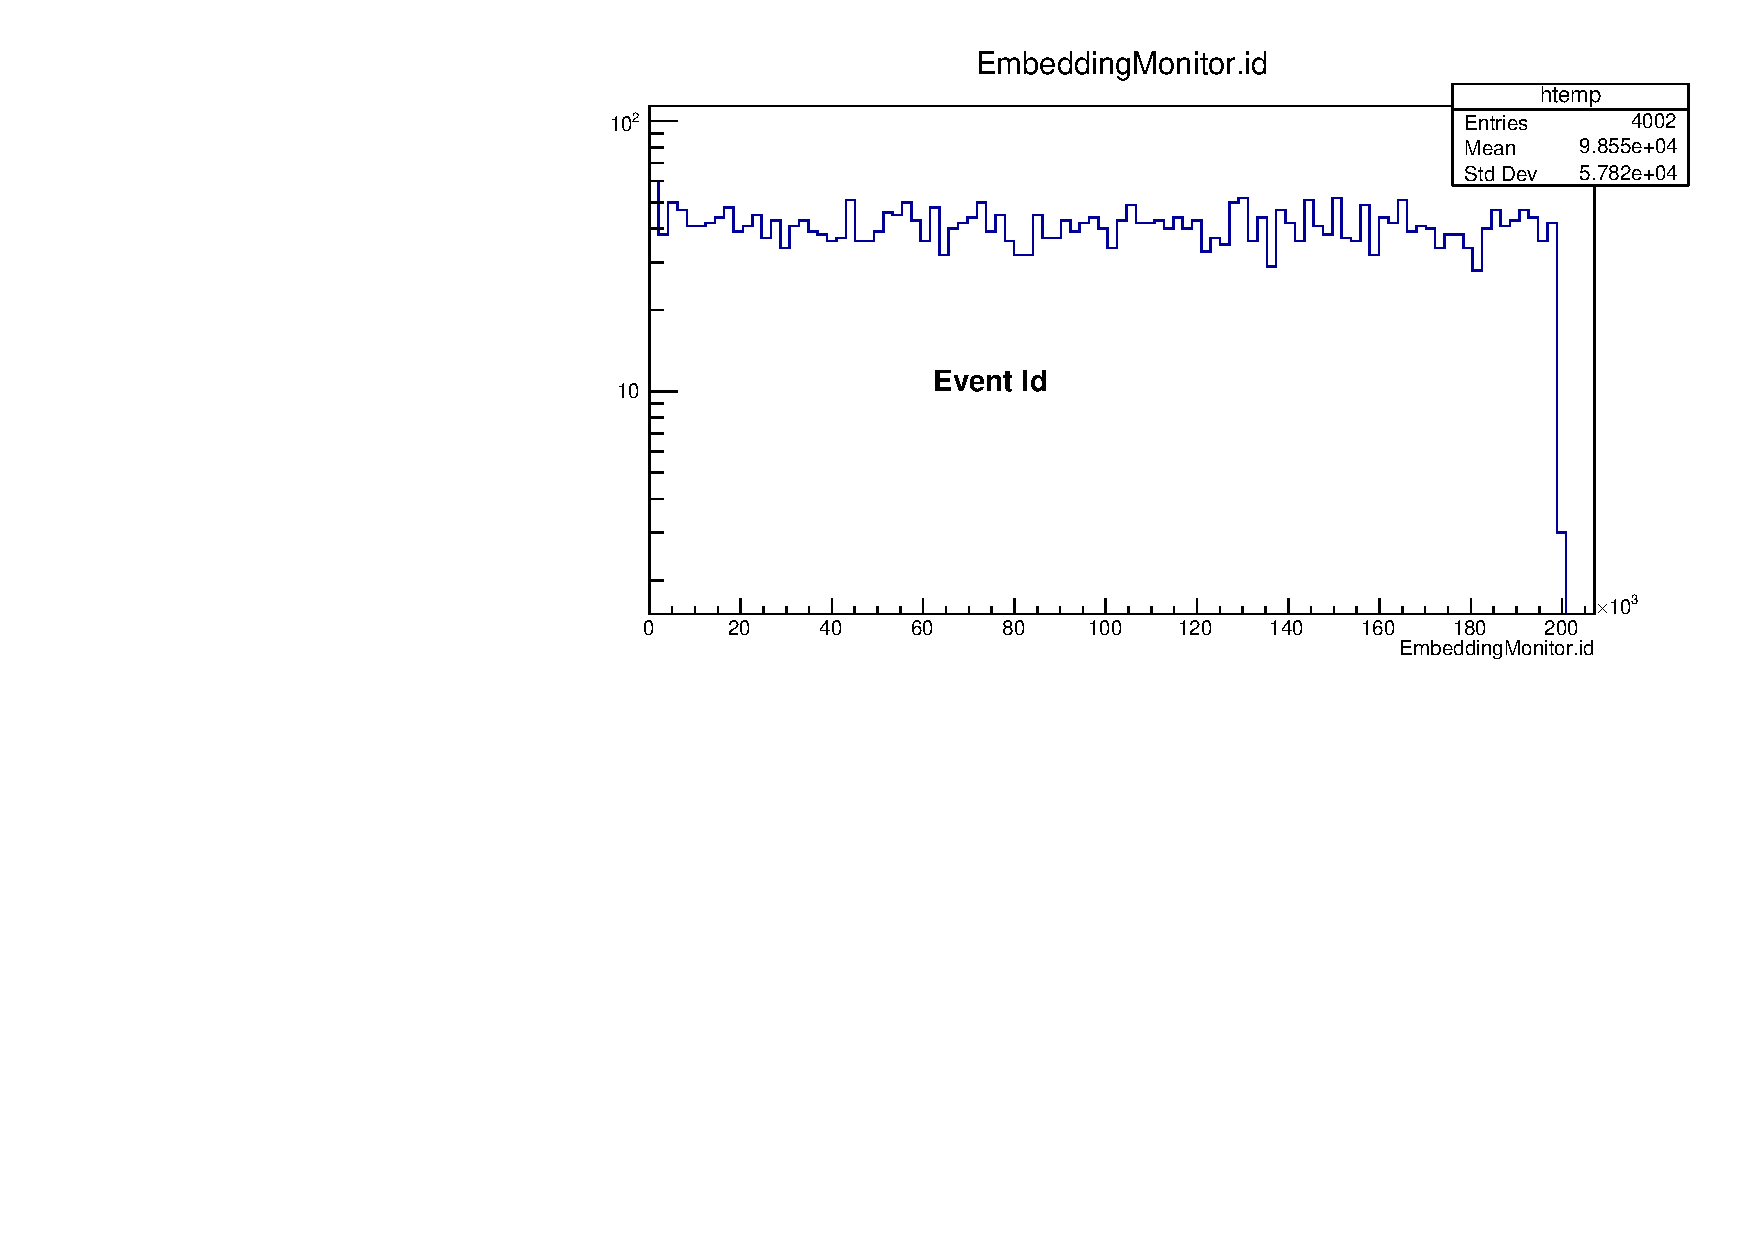
\includegraphics[width=1.\linewidth]{EmbeddingMonitorId.pdf}
           \end{figure}        
           \begin{figure}[H]
              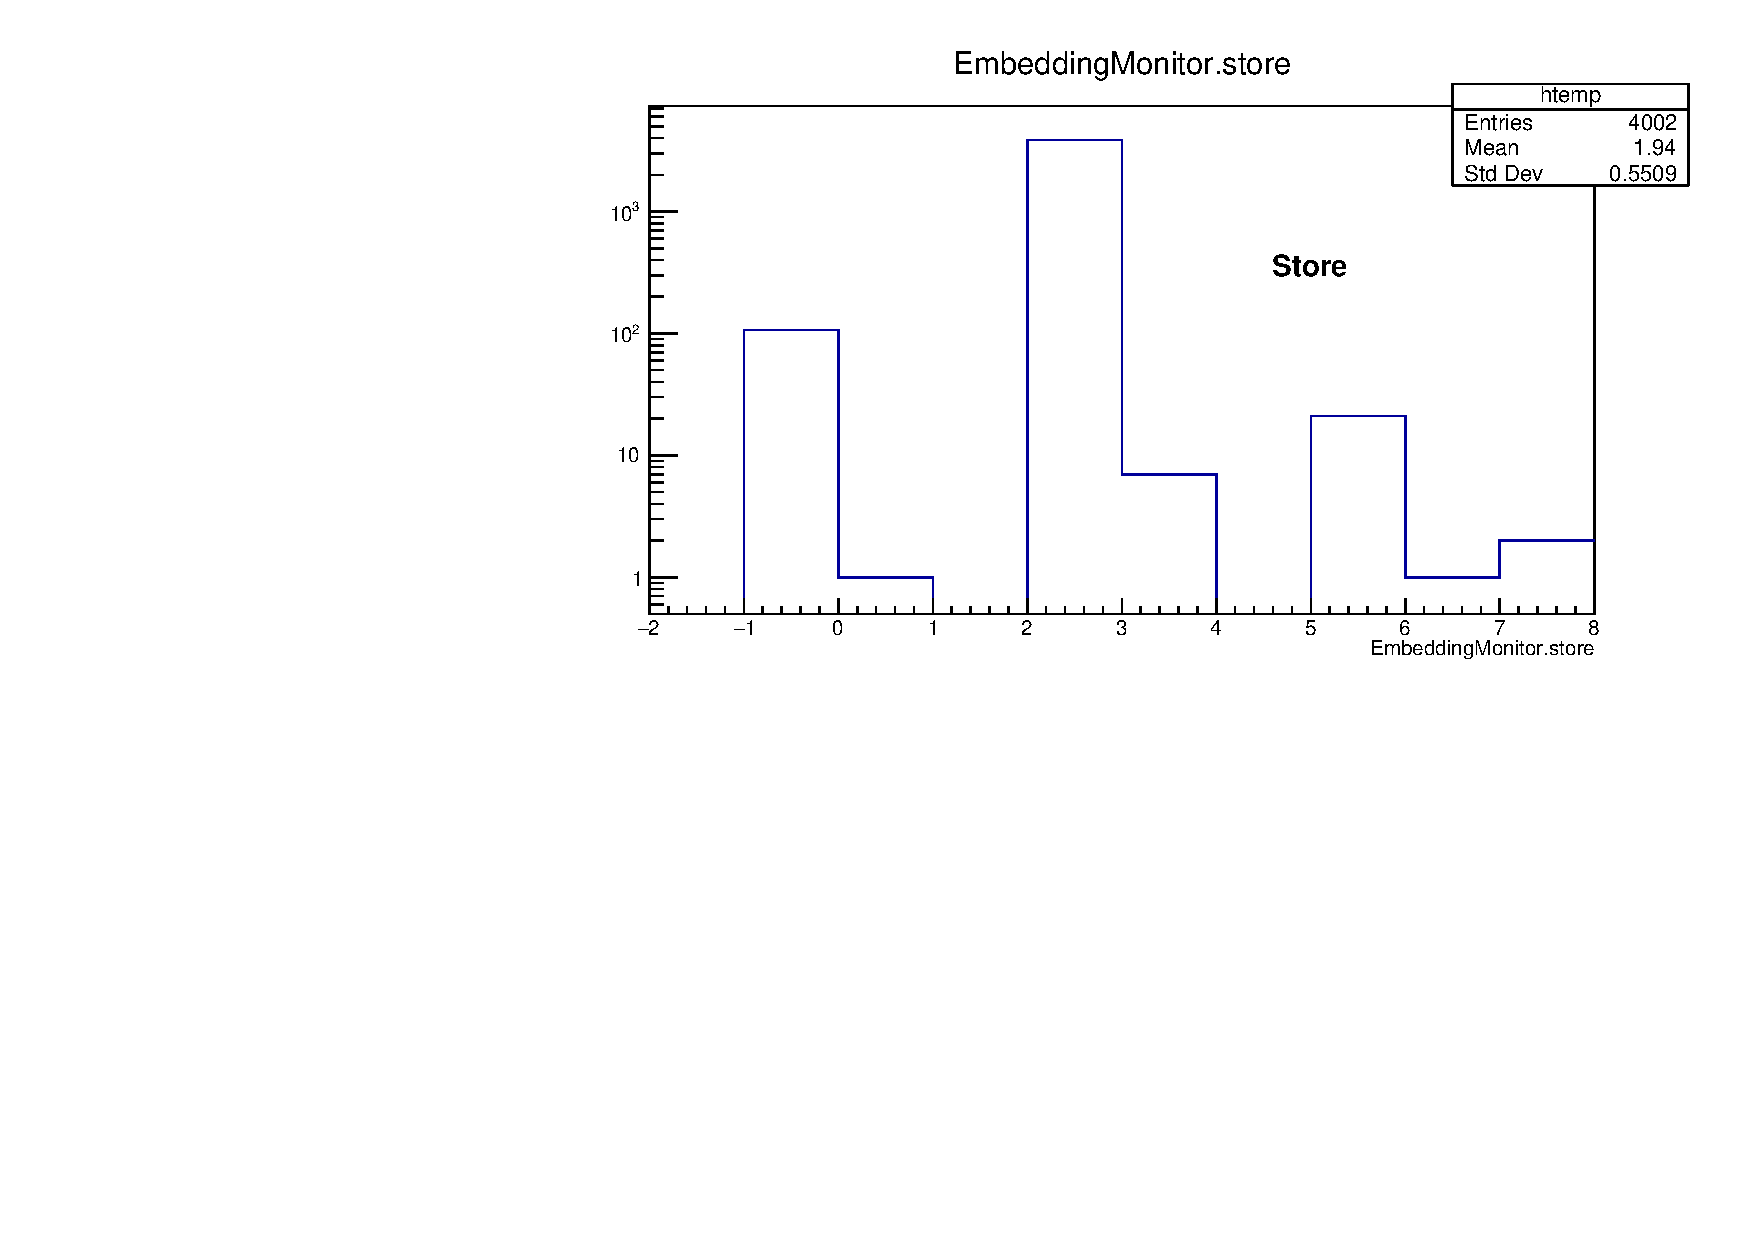
\includegraphics[width=1.\linewidth]{EmbeddingMonitorStore.pdf}
           \end{figure}

           \column{.49\textwidth}
            \begin{figure}[H]
              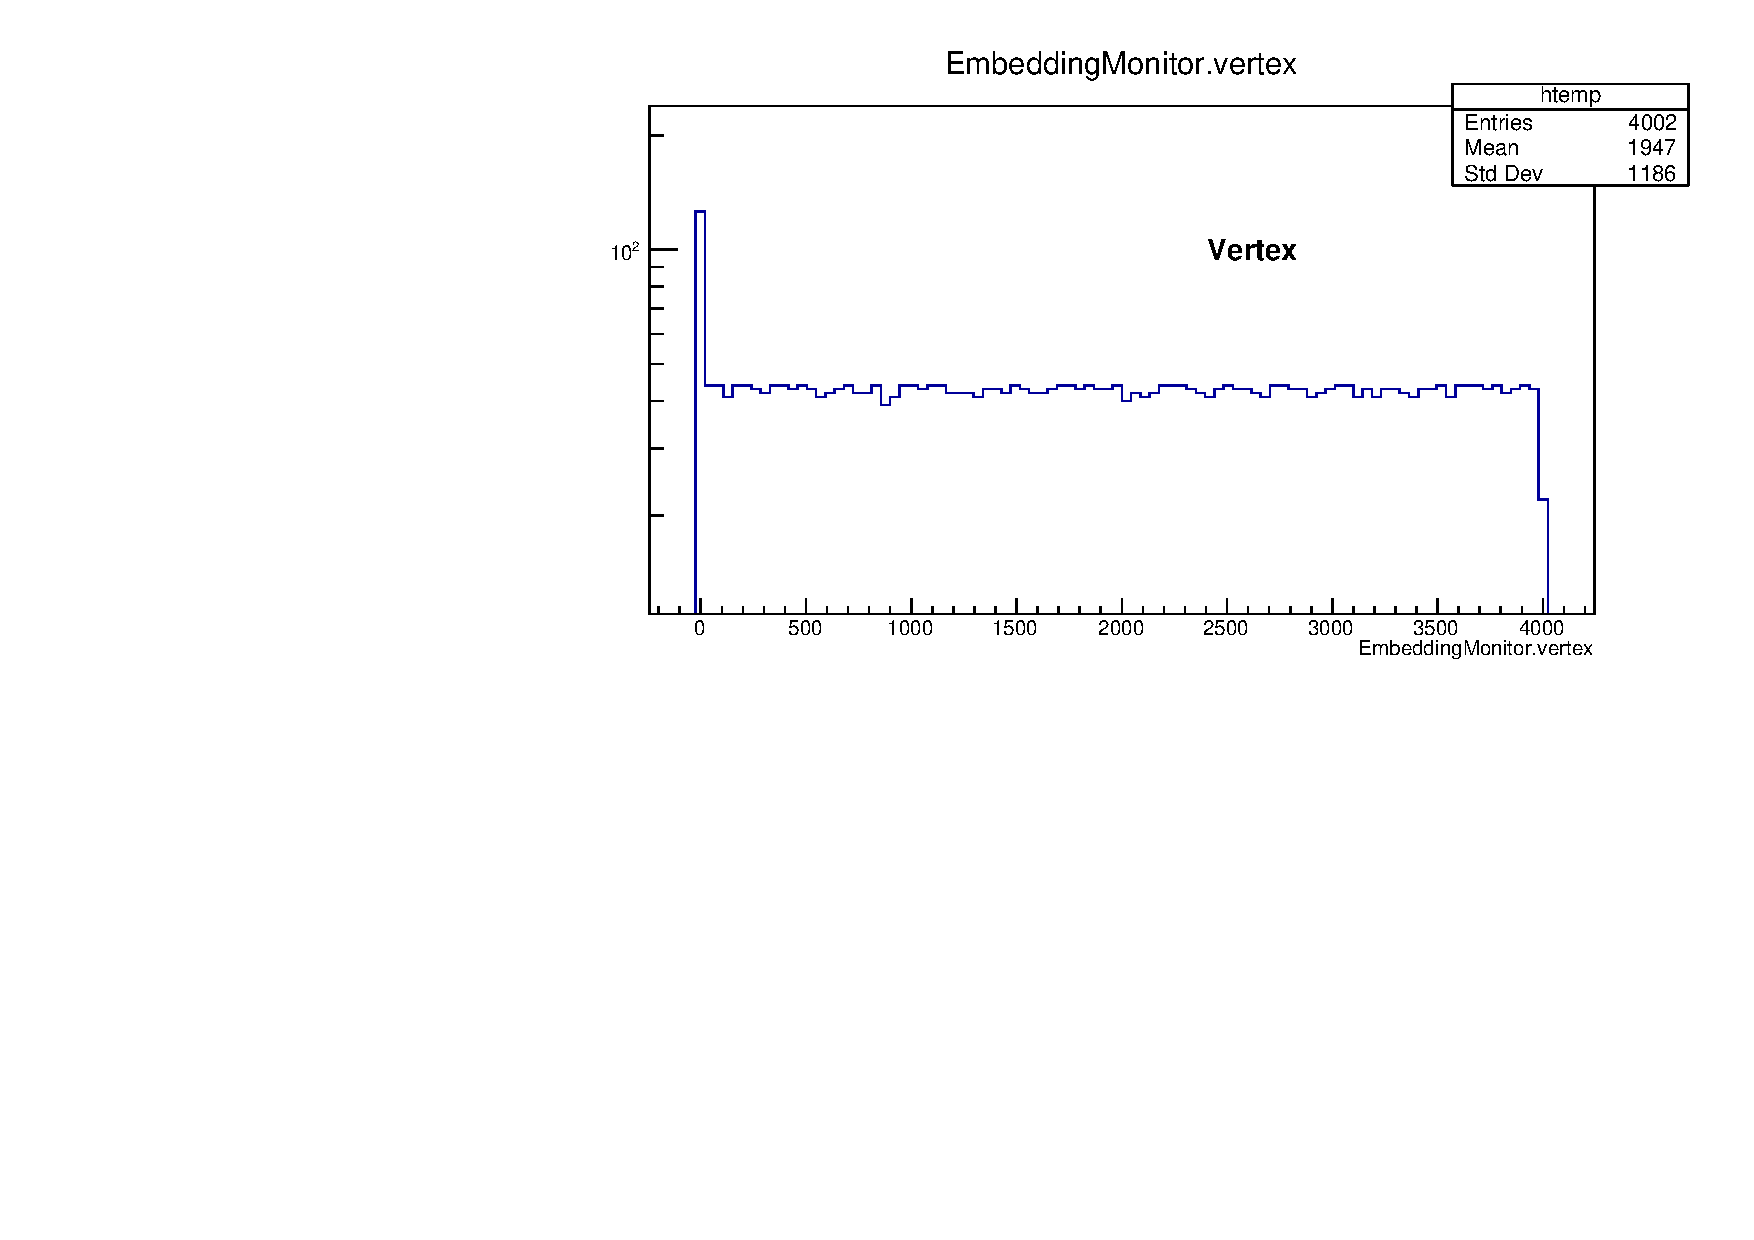
\includegraphics[width=1.\linewidth]{EmbeddingMonitorVertex.pdf}
           \end{figure}      
           \begin{figure}[H]
              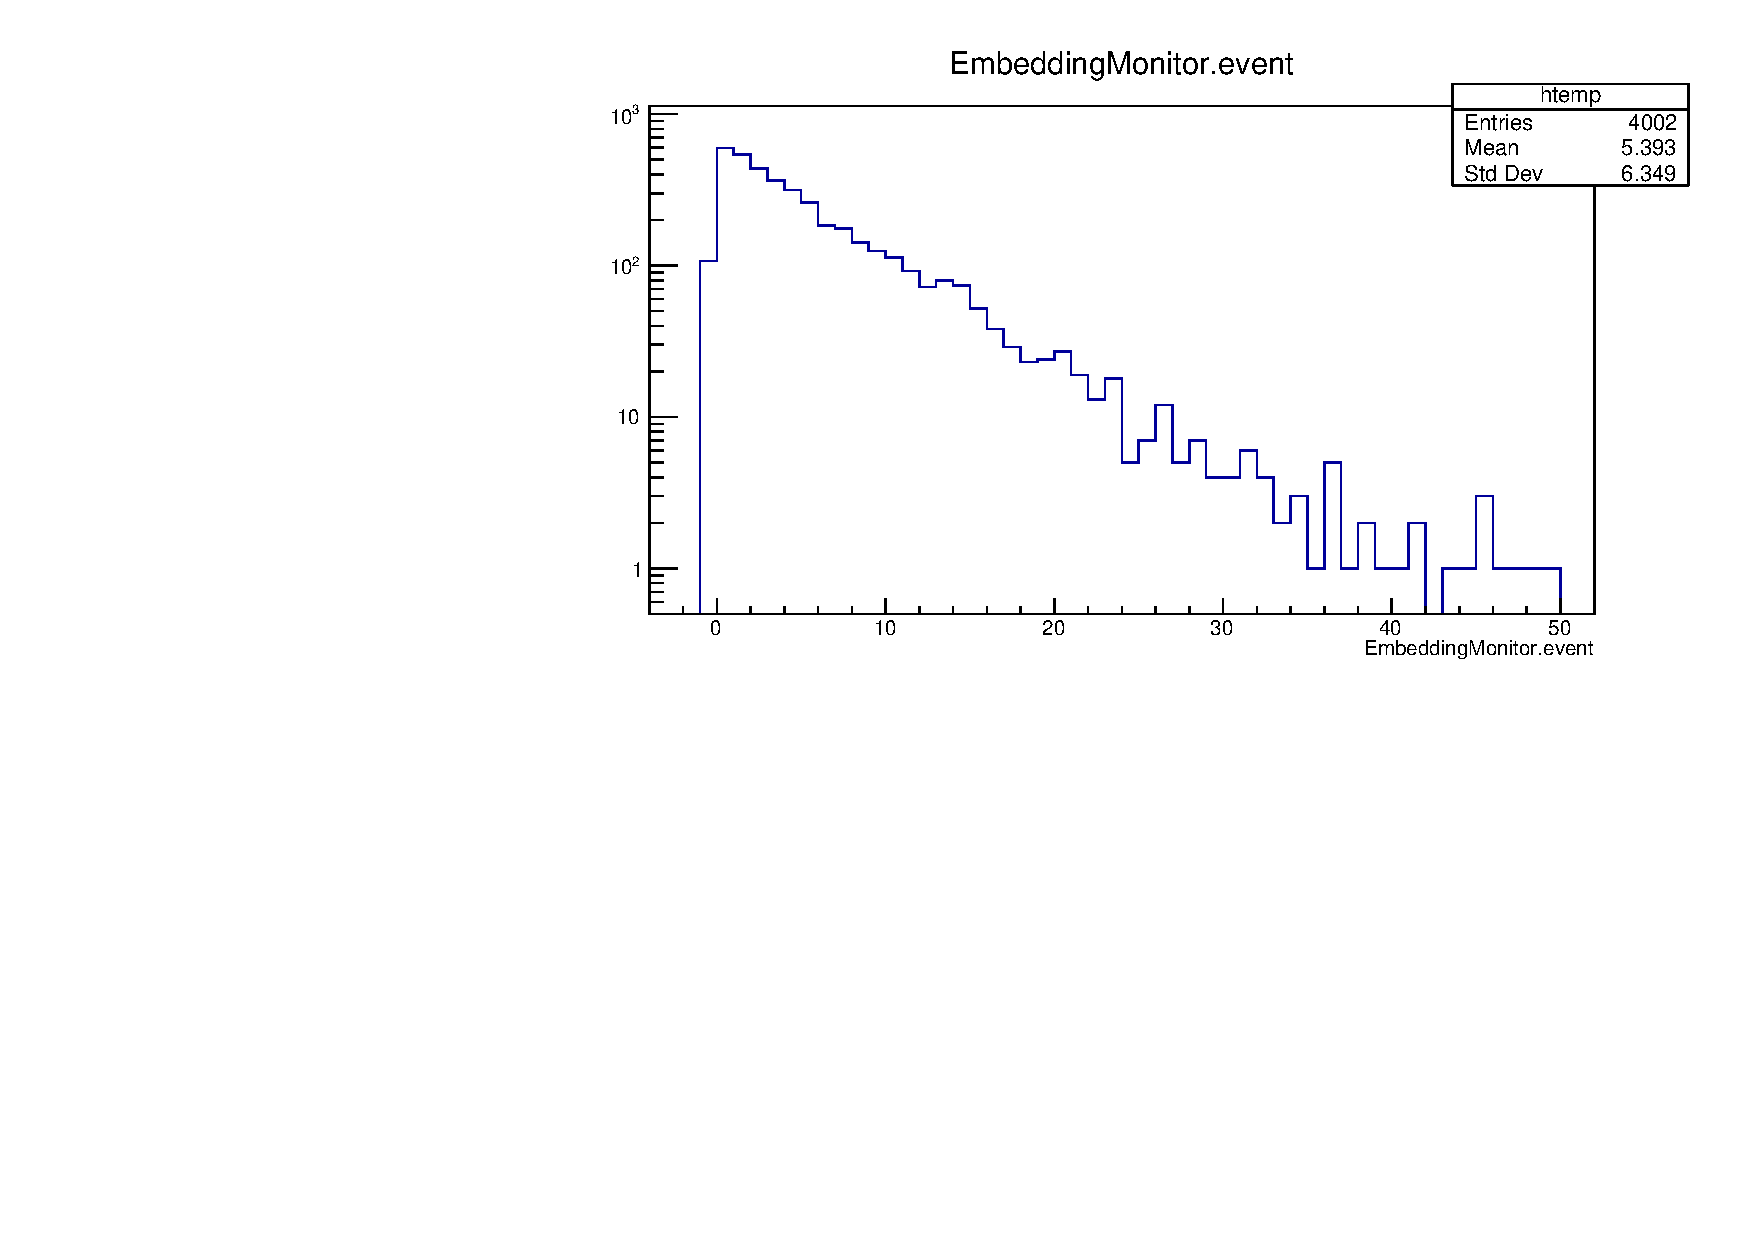
\includegraphics[width=1.\linewidth]{EmbeddingMonitorEvent.pdf}
           \end{figure}
         \end{columns}
         \end{block}
       \end{frame}

       \begin{frame}
         \frametitle{\bf \centering \footnotesize The Algorithm::Monitoring events with embedded products from $\Lambda^{0}$ decay}
          \begin{block}{\bf \centering \tiny To get info on different characteristics of particles}
         \begin{columns}[t]
           \column{.49\textwidth}
           \begin{figure}[H]
             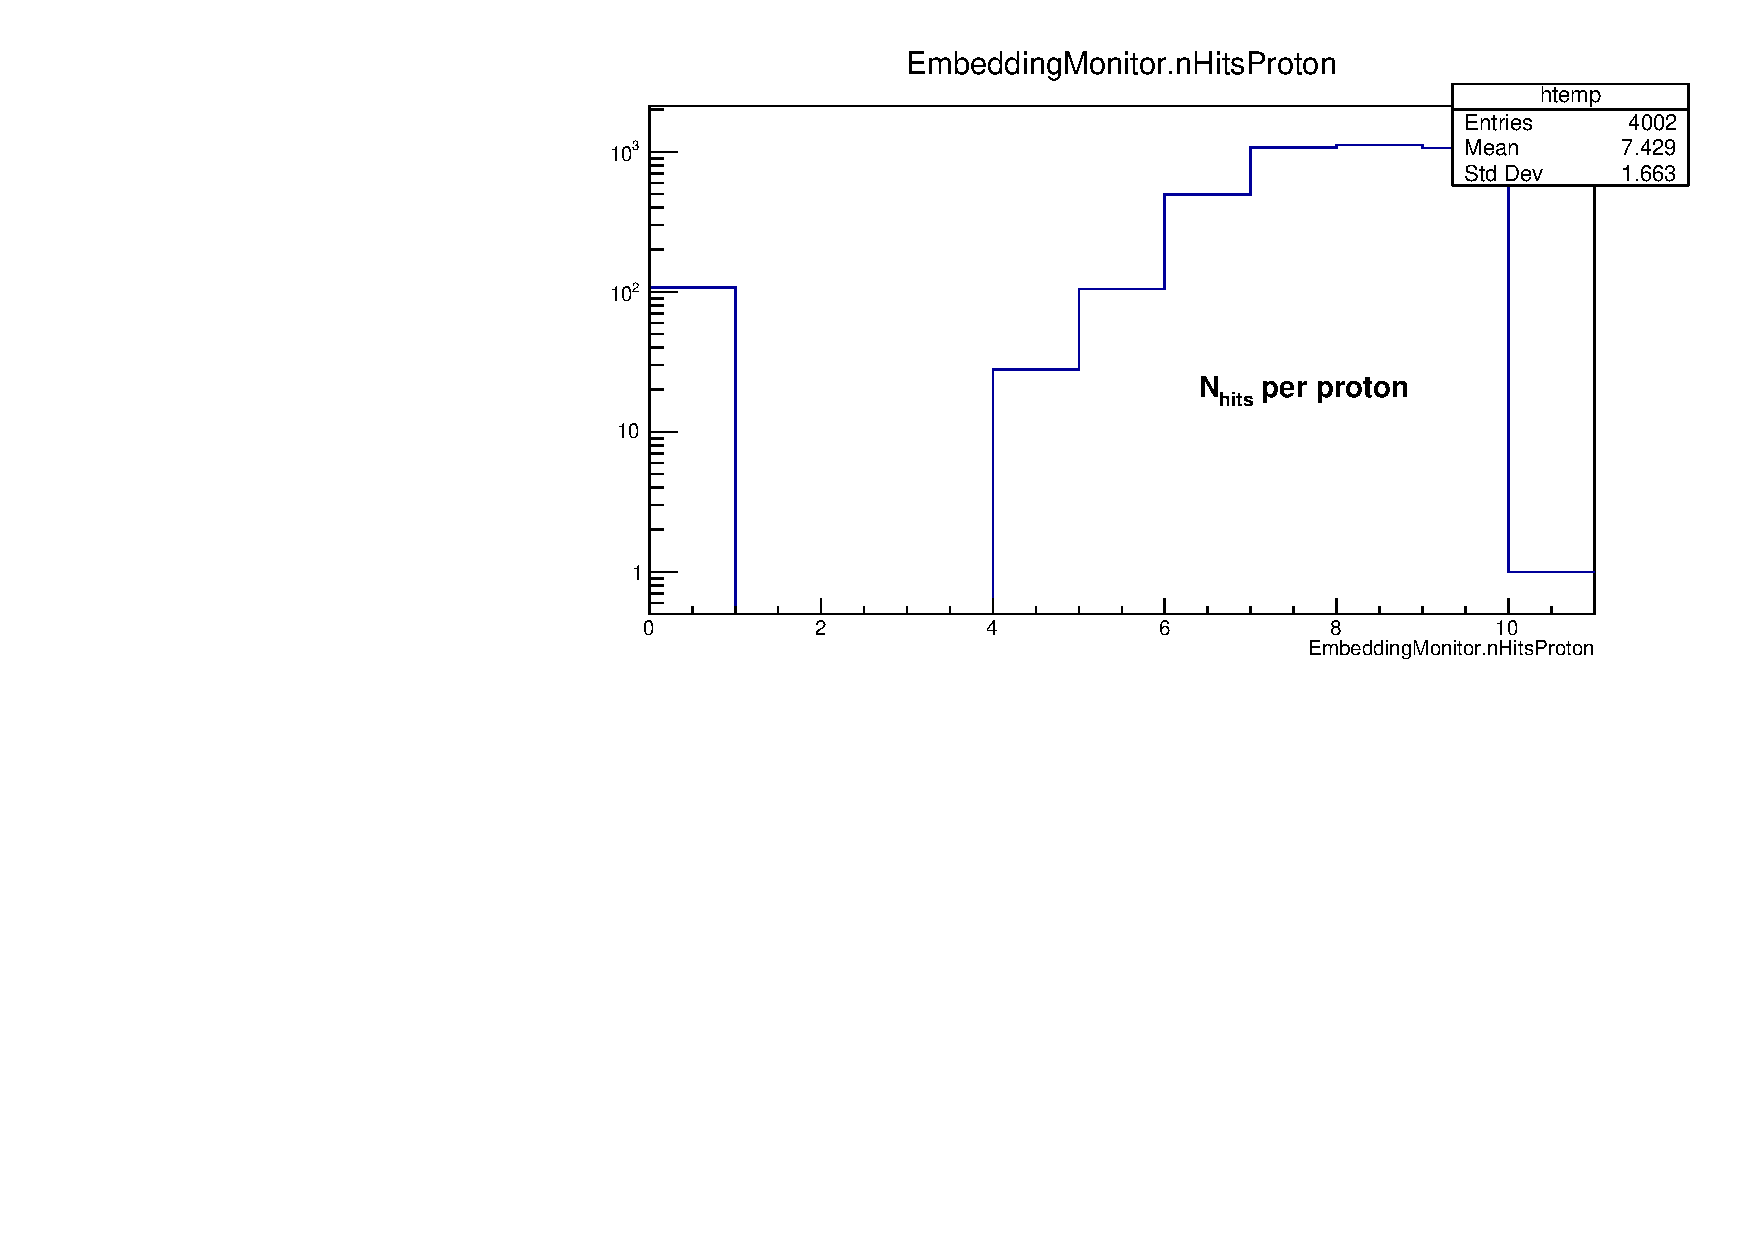
\includegraphics[width=1.\linewidth]{EmbeddingMonitorNhitsProton.pdf}
           \end{figure}        
           \begin{figure}[H]
              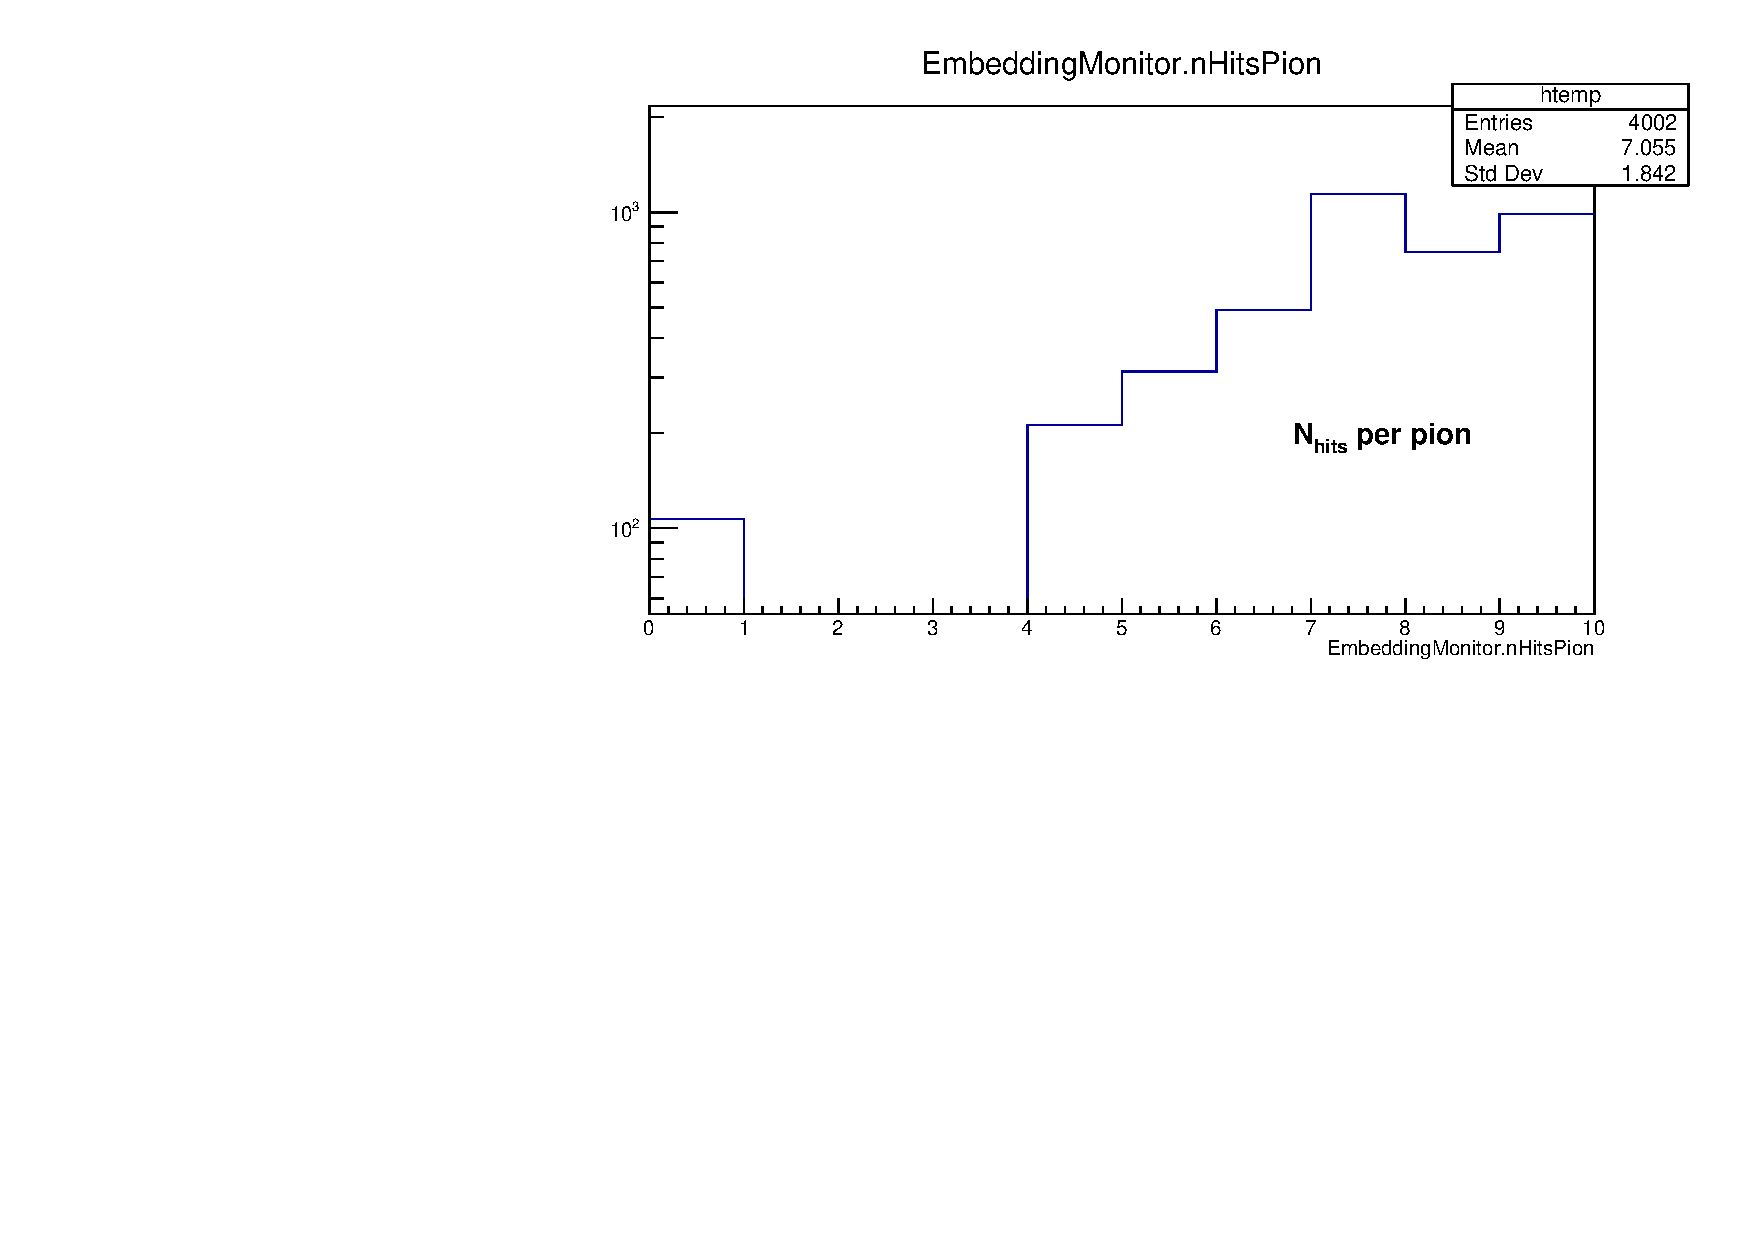
\includegraphics[width=1.\linewidth]{EmbeddingMonitorNhitsPion.pdf}
           \end{figure}

           \column{.49\textwidth}
            \begin{figure}[H]
              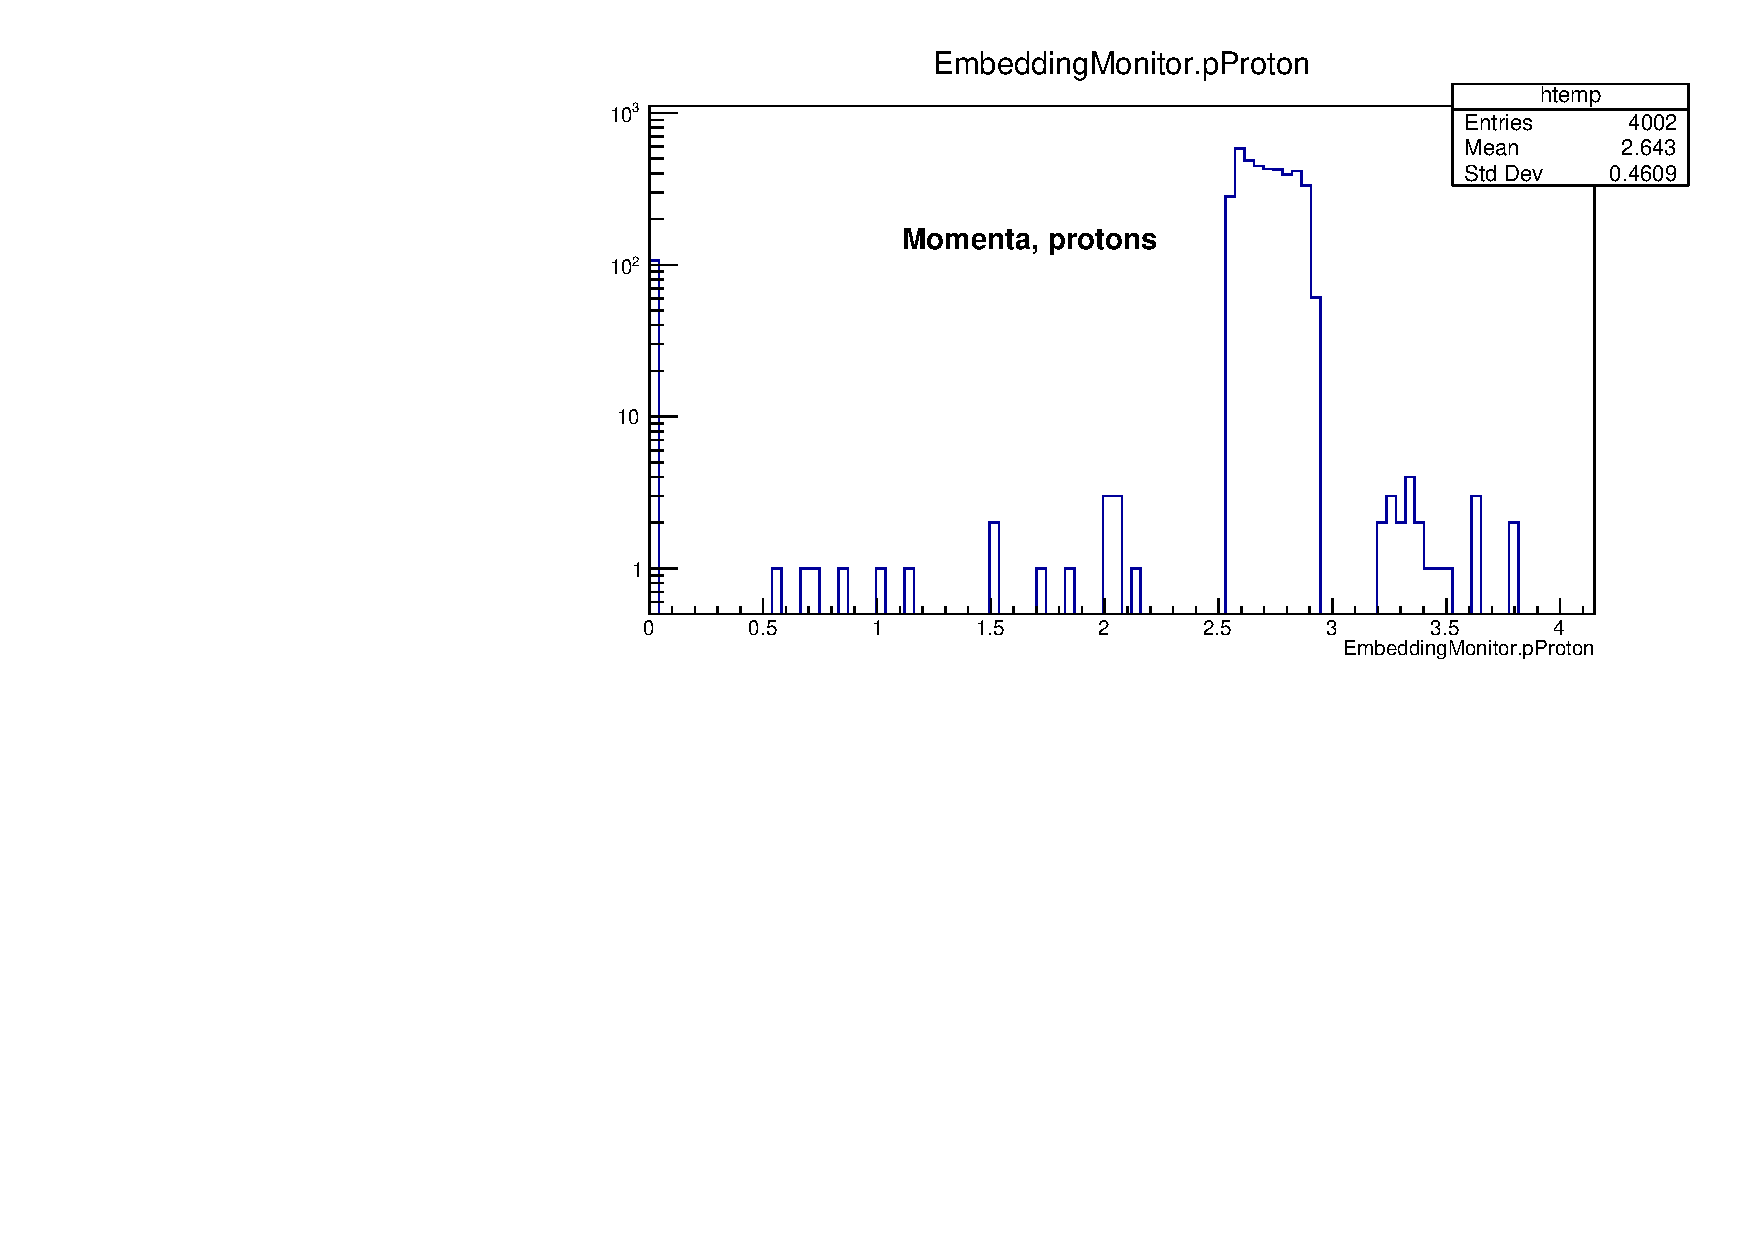
\includegraphics[width=1.\linewidth]{EmbeddingMonitorMomentaProton.pdf}
           \end{figure}      
           \begin{figure}[H]
              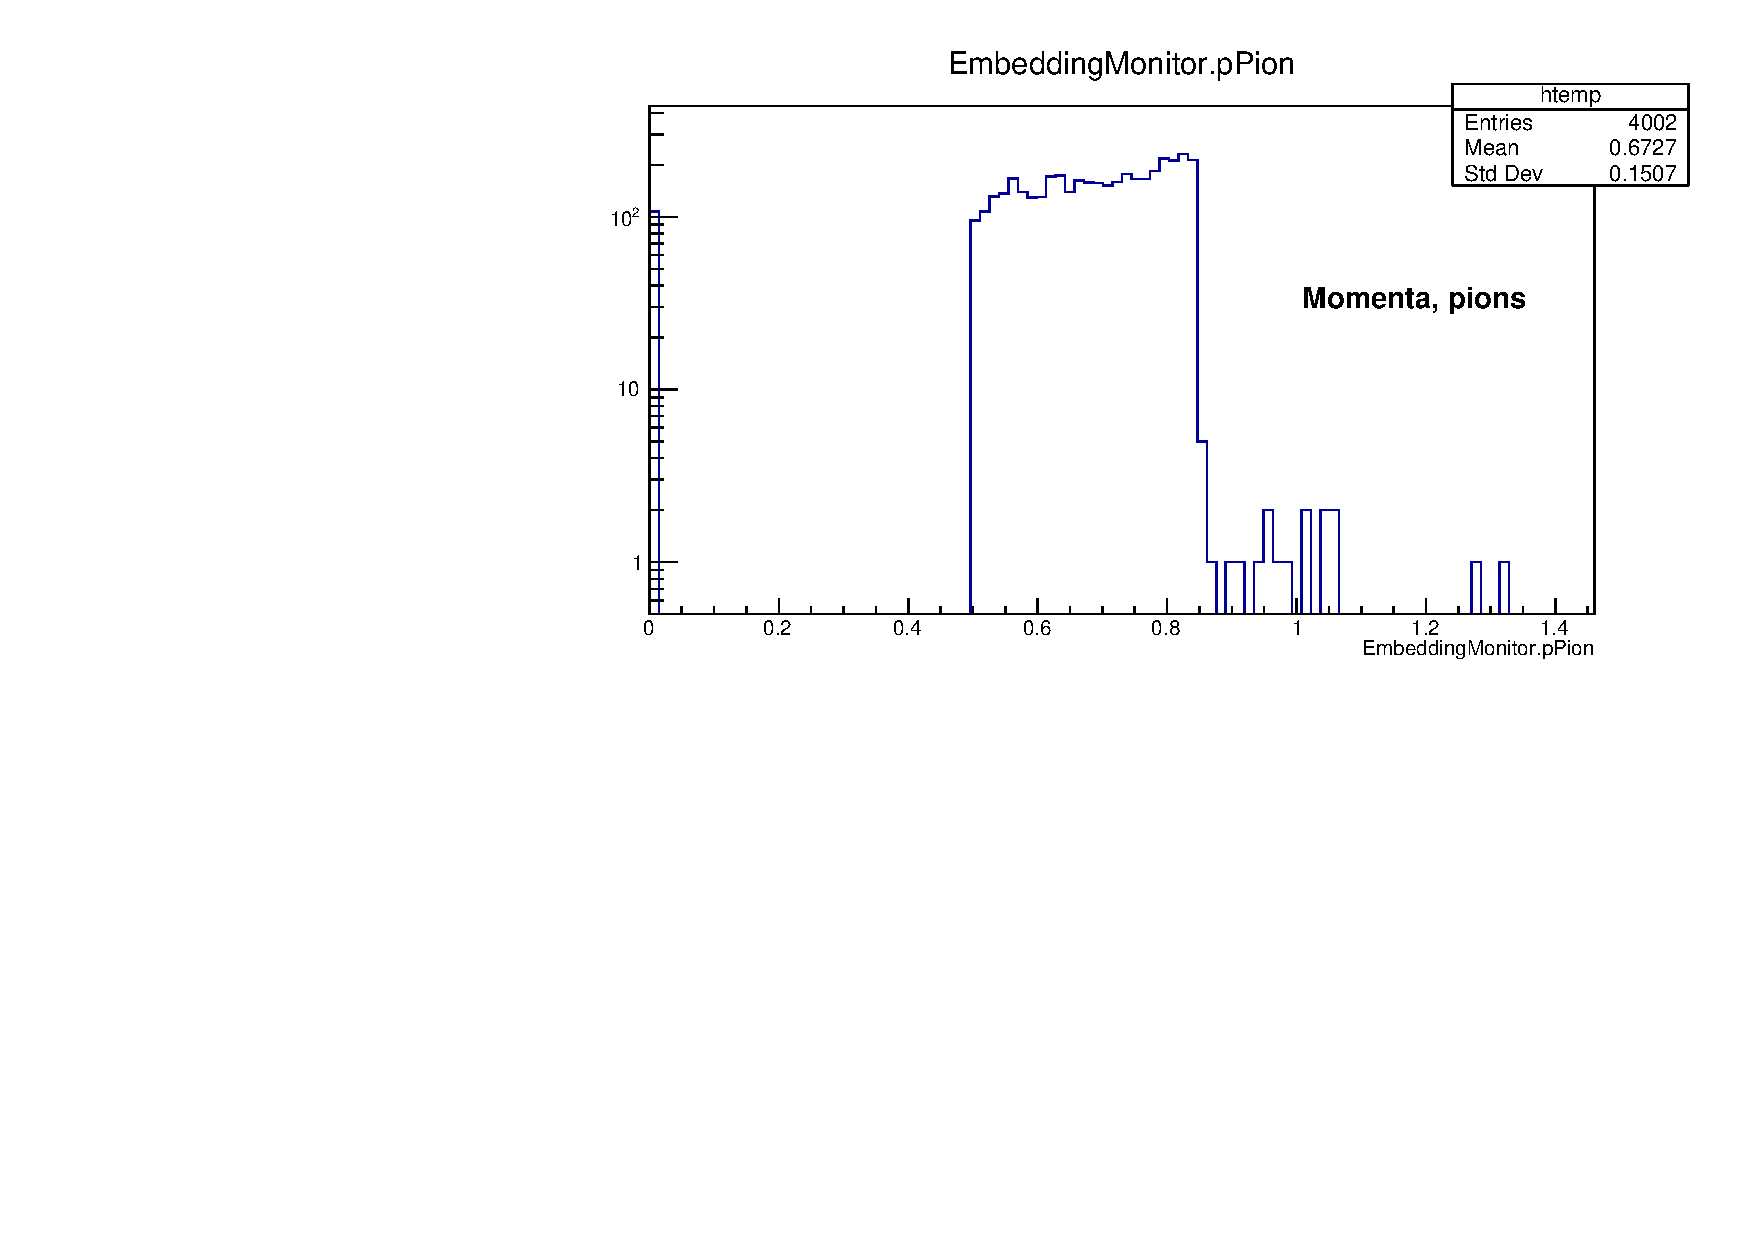
\includegraphics[width=1.\linewidth]{EmbeddingMonitorMomentaPion.pdf}
           \end{figure}
         \end{columns}
         \end{block}
       \end{frame}

       \begin{frame}
         \frametitle{\bf \centering \footnotesize The Algorithm::Creating digits from $\Lambda^{0}$ decay products}       
         \bf
         \vskip -0.75cm
         \begin{columns}[t]
           \column{.49\textwidth}
            \begin{block}{}
           \begin{figure}[H]
             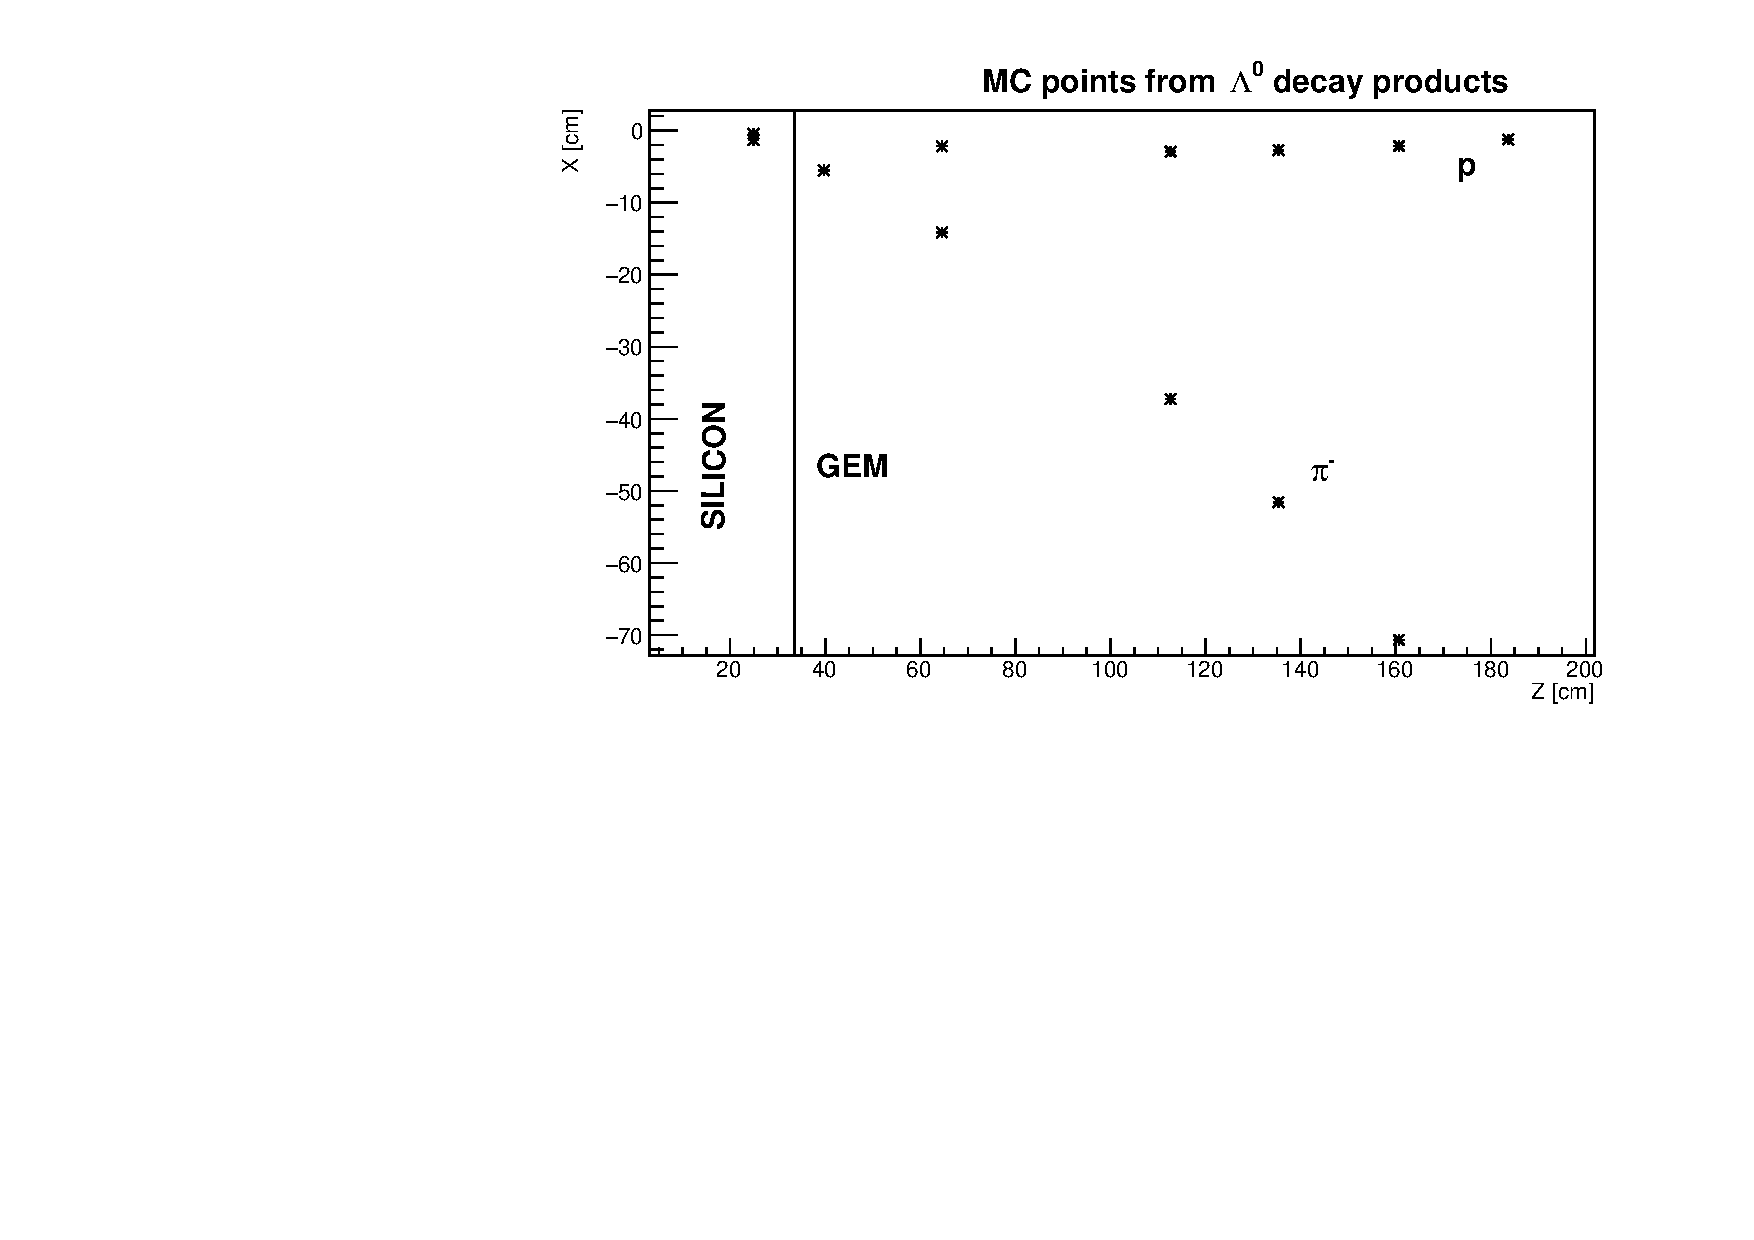
\includegraphics[width=1.\linewidth]{EmbeddingMCPoints.pdf}
             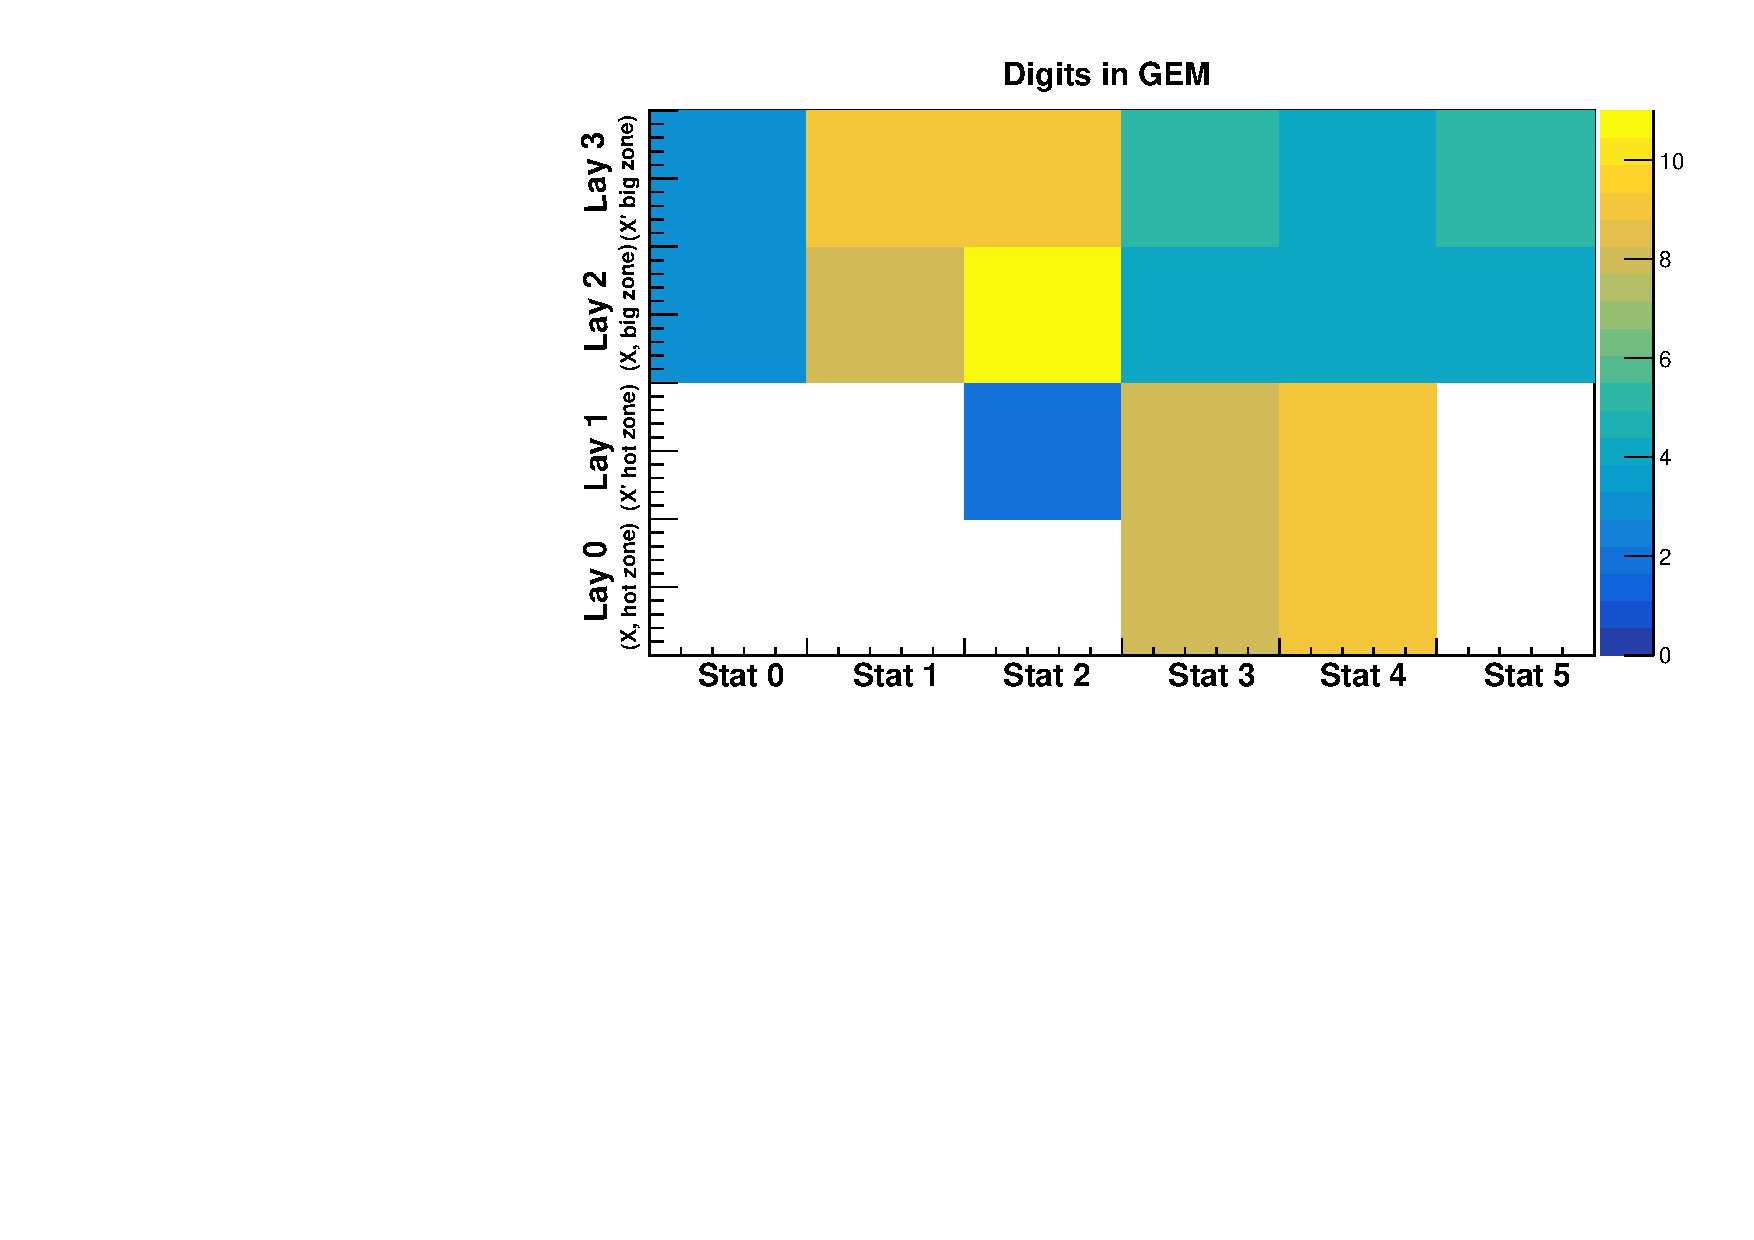
\includegraphics[width=1.\linewidth]{EmbeddingGemDigits.pdf}
            \end{figure}
            \end{block}
            \vskip -0.3cm
            \begin{block}{}
              \tiny
              Clusters with $N_{strips} > 5$ produce hits being reconstructed with a slightly pure efficiency
              (see next slides)
            \end{block}
            \column{.49\textwidth}
            \begin{block}{}
             \begin{figure}[H]
             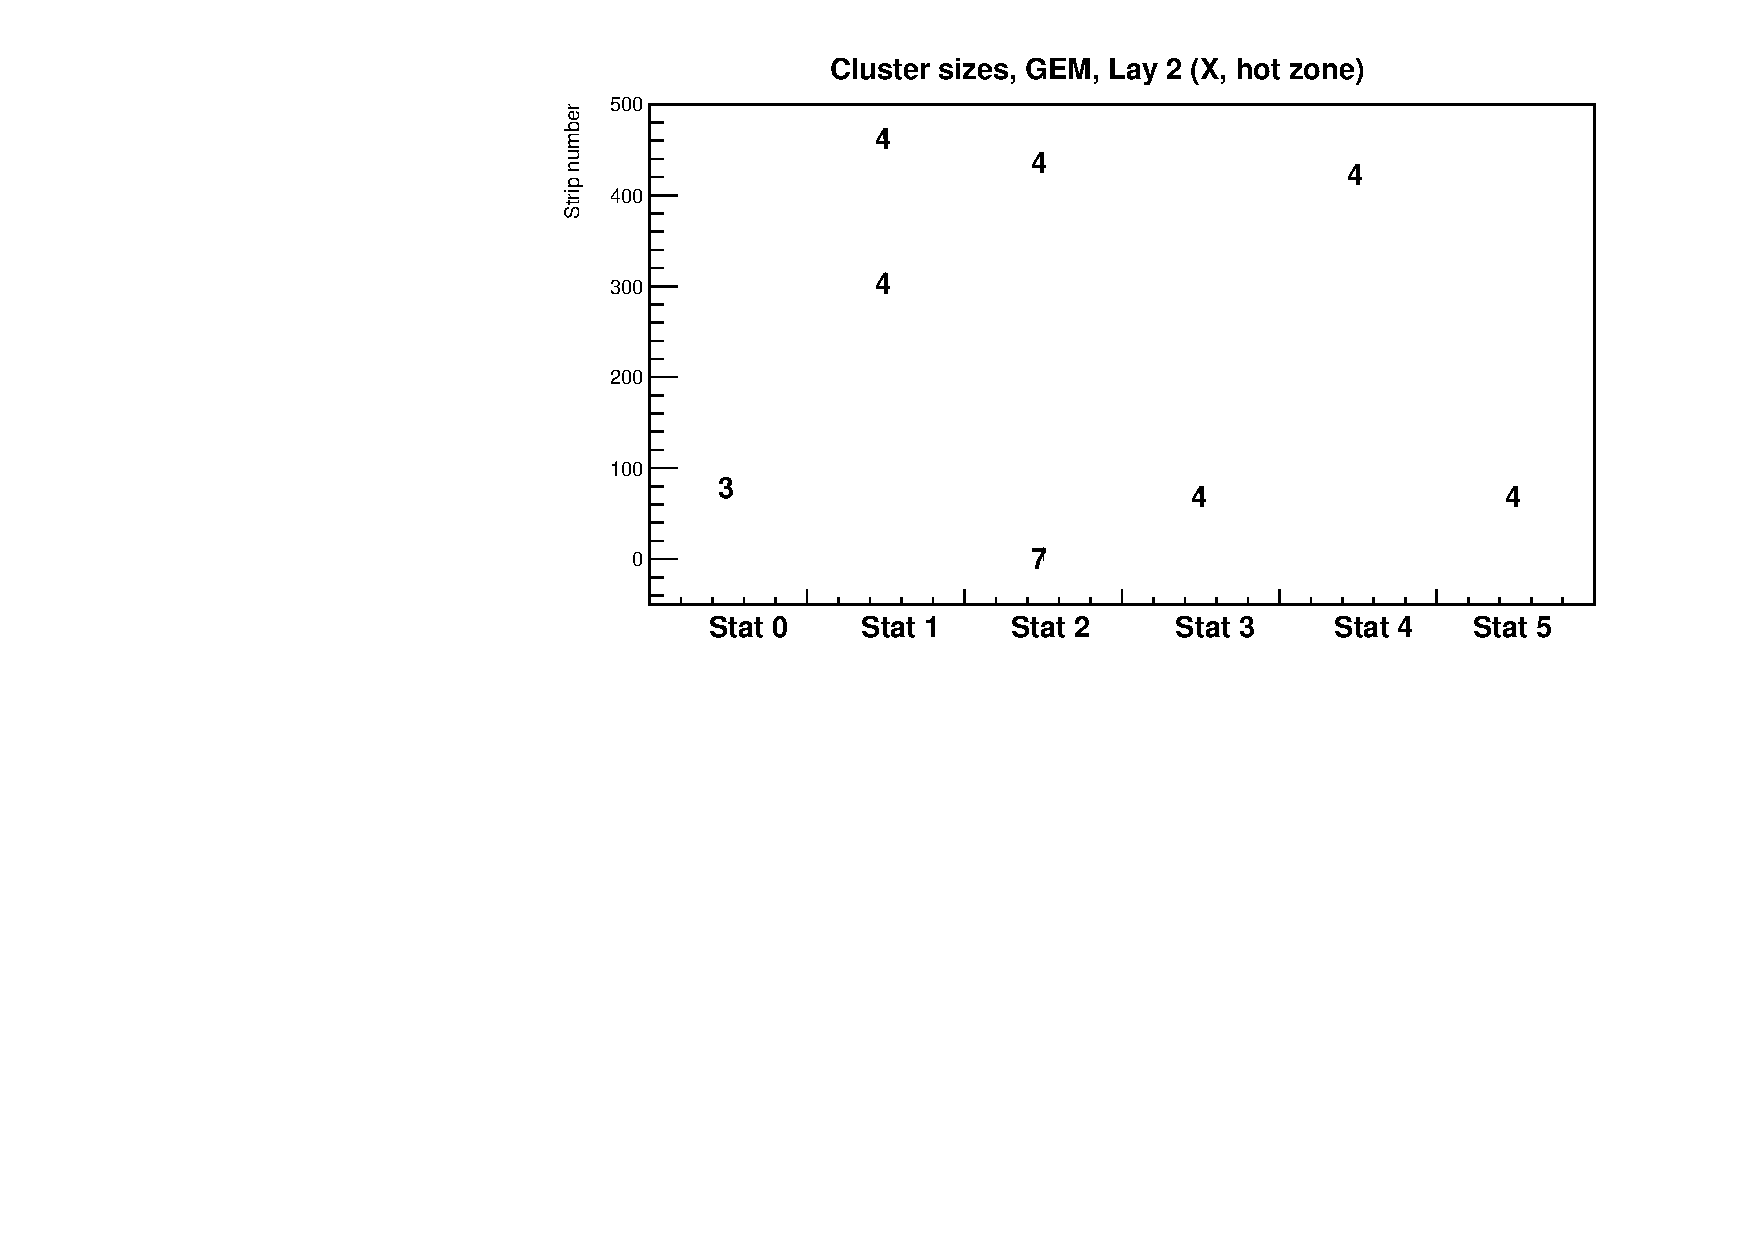
\includegraphics[width=1.\linewidth]{EmbeddingClustersLay2.pdf}
             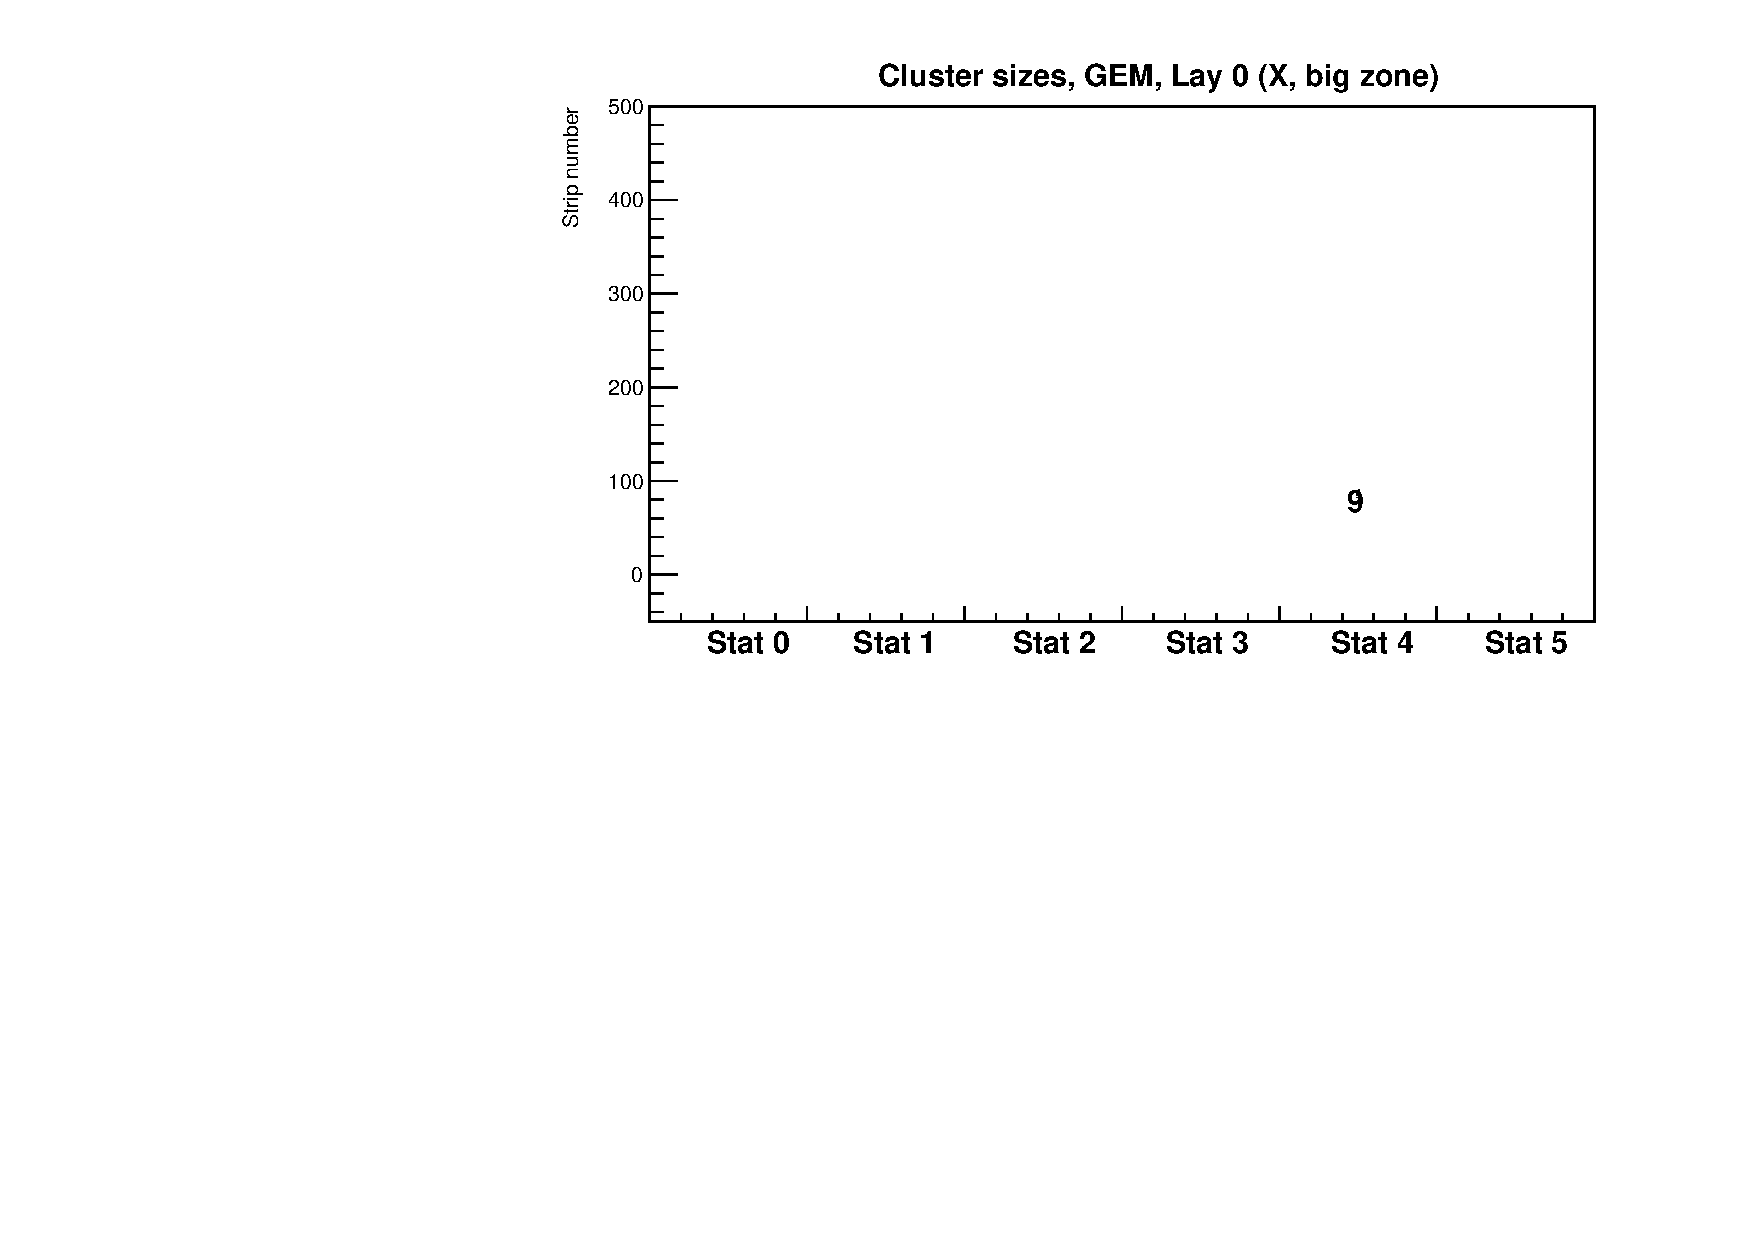
\includegraphics[width=1.\linewidth]{EmbeddingClustersLay0.pdf}
              \end{figure}
            \end{block}
            \vskip -0.3cm
            \begin{block}{}
              \tiny
              \begin{itemize}
              \item Equal amplitudes for each strip in the cluster assumed
              \item Scenarios with different Gaussian smearing are being tested 
              \end{itemize}
            \end{block}
          \end{columns}
       \end{frame}

       \begin{frame}[fragile]        
         \frametitle{\bf \centering \tiny The Algorithm::Doing correspondence between digits from $\Lambda^{0}$ decay products to a channel and a serial number of ADC}
         \vskip -0.75cm
         \bf
         \begin{columns}[t]
           \column{.49\textwidth}

           \begin{block}{\bf \centering Central Tracker, mappings}
             \tiny
\begin{verbatim}
                          GEM
// GEM_id: the second digit 0=left, 1=right;
// Module: 0=00 (mod0,hotZone), 1=01 (mod0,bigZone),
// 2=10 (mod1,hotZone), 3=11 (mod1,bigZone)
   Serial    Ch_lo    Ch_hi   GEM_id  Station  Module
=====================================================
0x76CD410     1024     2047      110      0       0
0x76C8320        0     2047      110      0       1
0x76CB9C0        0     2047      111      0       3
0x76CA266     1024     2047      111      0       2
0x76D08B9      512      767      110      0       1
0x76D4D2B        0     1023      100      1       2
0x76D5044        0     2047      100      1       3
...         
\end{verbatim}
\tiny
\begin{verbatim}
                        SILICON
// Station: 0 - vertex (near), 1 - vertex(far), 
// 2 - Forward detector
//Layer: 0 - vertical strips, 1 - sloped strips
Serial    Ch_lo    Ch_hi   GEO_mod   Layer  Station
====================================================
0x80BCBFC   42       46      0       0        2
0x80BCBFC   37       41      0       1        2
0x80BCBFC   32       36      1       0        2
0x80BCBFC   26       30      1       1        2
0x80BCBFC   16       20      2       0        2
0x80BCBFC   21       25      2       1        2
0x80BCBFC    5        9      3       0        2
... 
\end{verbatim}
\end{block}

           \column{.49\textwidth}
           \begin{block}{\bf \centering BmnStripDigit (GEM or SILICON)}
\begin{verbatim}
      Int_t fStation;
      Int_t fModule;
      Int_t fStripLayer;
      Int_t fStripNumber;
      Double_t fStripSignal;
\end{verbatim}           
           \end{block}
           \begin{block}{}
             {\scriptsize \color{blue} Direct problem: ADC-digits from DAQ $\rightarrow$ Physical digits (decoding)} \\
             {\scriptsize \color{red} Inverse problem: Physical digits $\rightarrow$ Incorporation to ADC-digits (embedding) + direct problem}
           \end{block}
           \vskip -.3cm
           \begin{block}{}
             \footnotesize Operating dig. info one has to define corresponding channels \& serials using mappings  
           \end{block}
 \end{columns}
\end{frame}

       
      \begin{frame}
        \frametitle{\bf \centering DST used as a start point for the procedure}
        \begin{columns}[t]
          \column{.49\textwidth}
          \begin{block}{\bf \centering Reconstructed $Z_{vertex}$ over all file}
            \begin{figure}[H]
              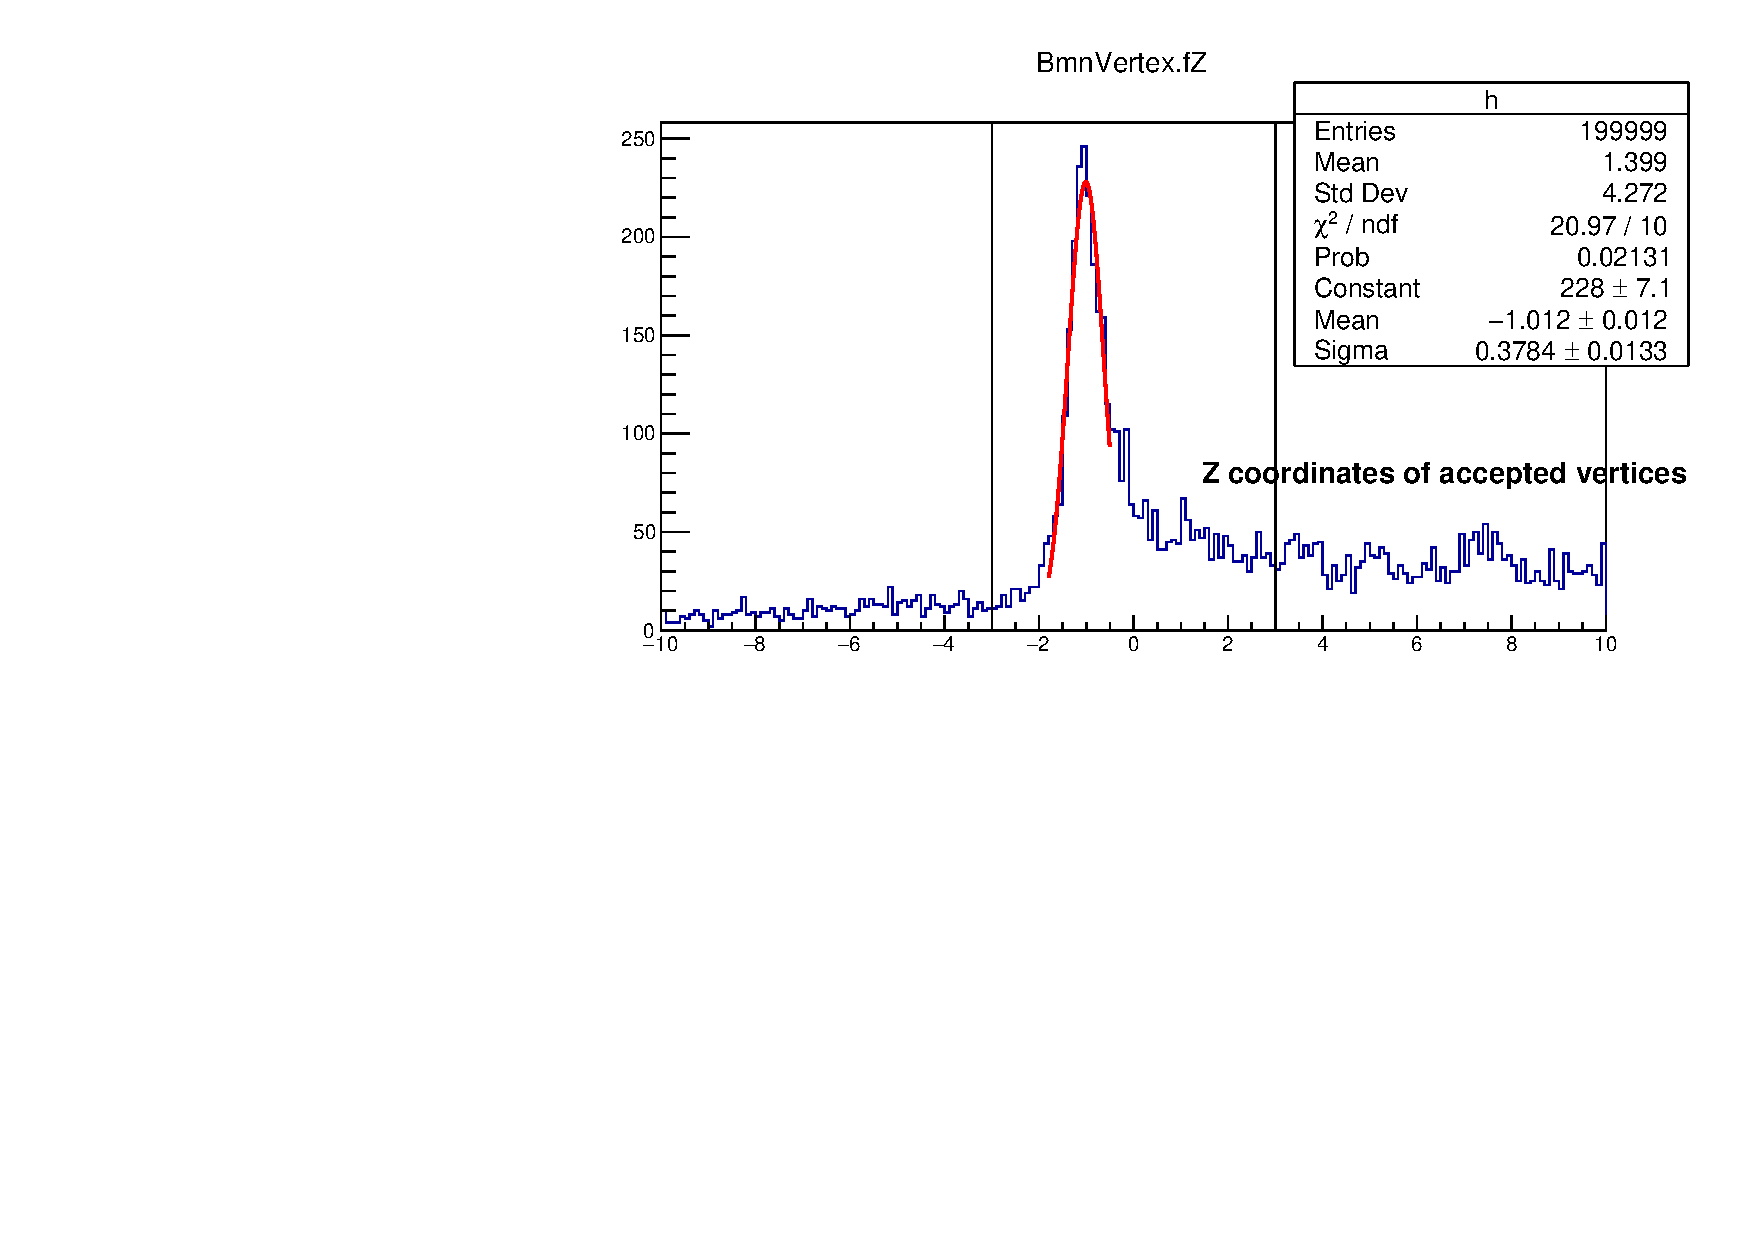
\includegraphics[width=1.\linewidth]{EmbeddingVertexZAll.pdf}
            \end{figure}
          \end{block}
          \begin{block}{}
            \bf
            \begin{itemize}
            \item bmndst\_4649.root, ArAl-interactions
            \item {\color{red} Old (not recently improved) algorithm of vertex finder used}
            \end{itemize}
          \end{block}
          
          \column{.49\textwidth}
           \begin{block}{\bf \centering }
            \begin{figure}[H]
              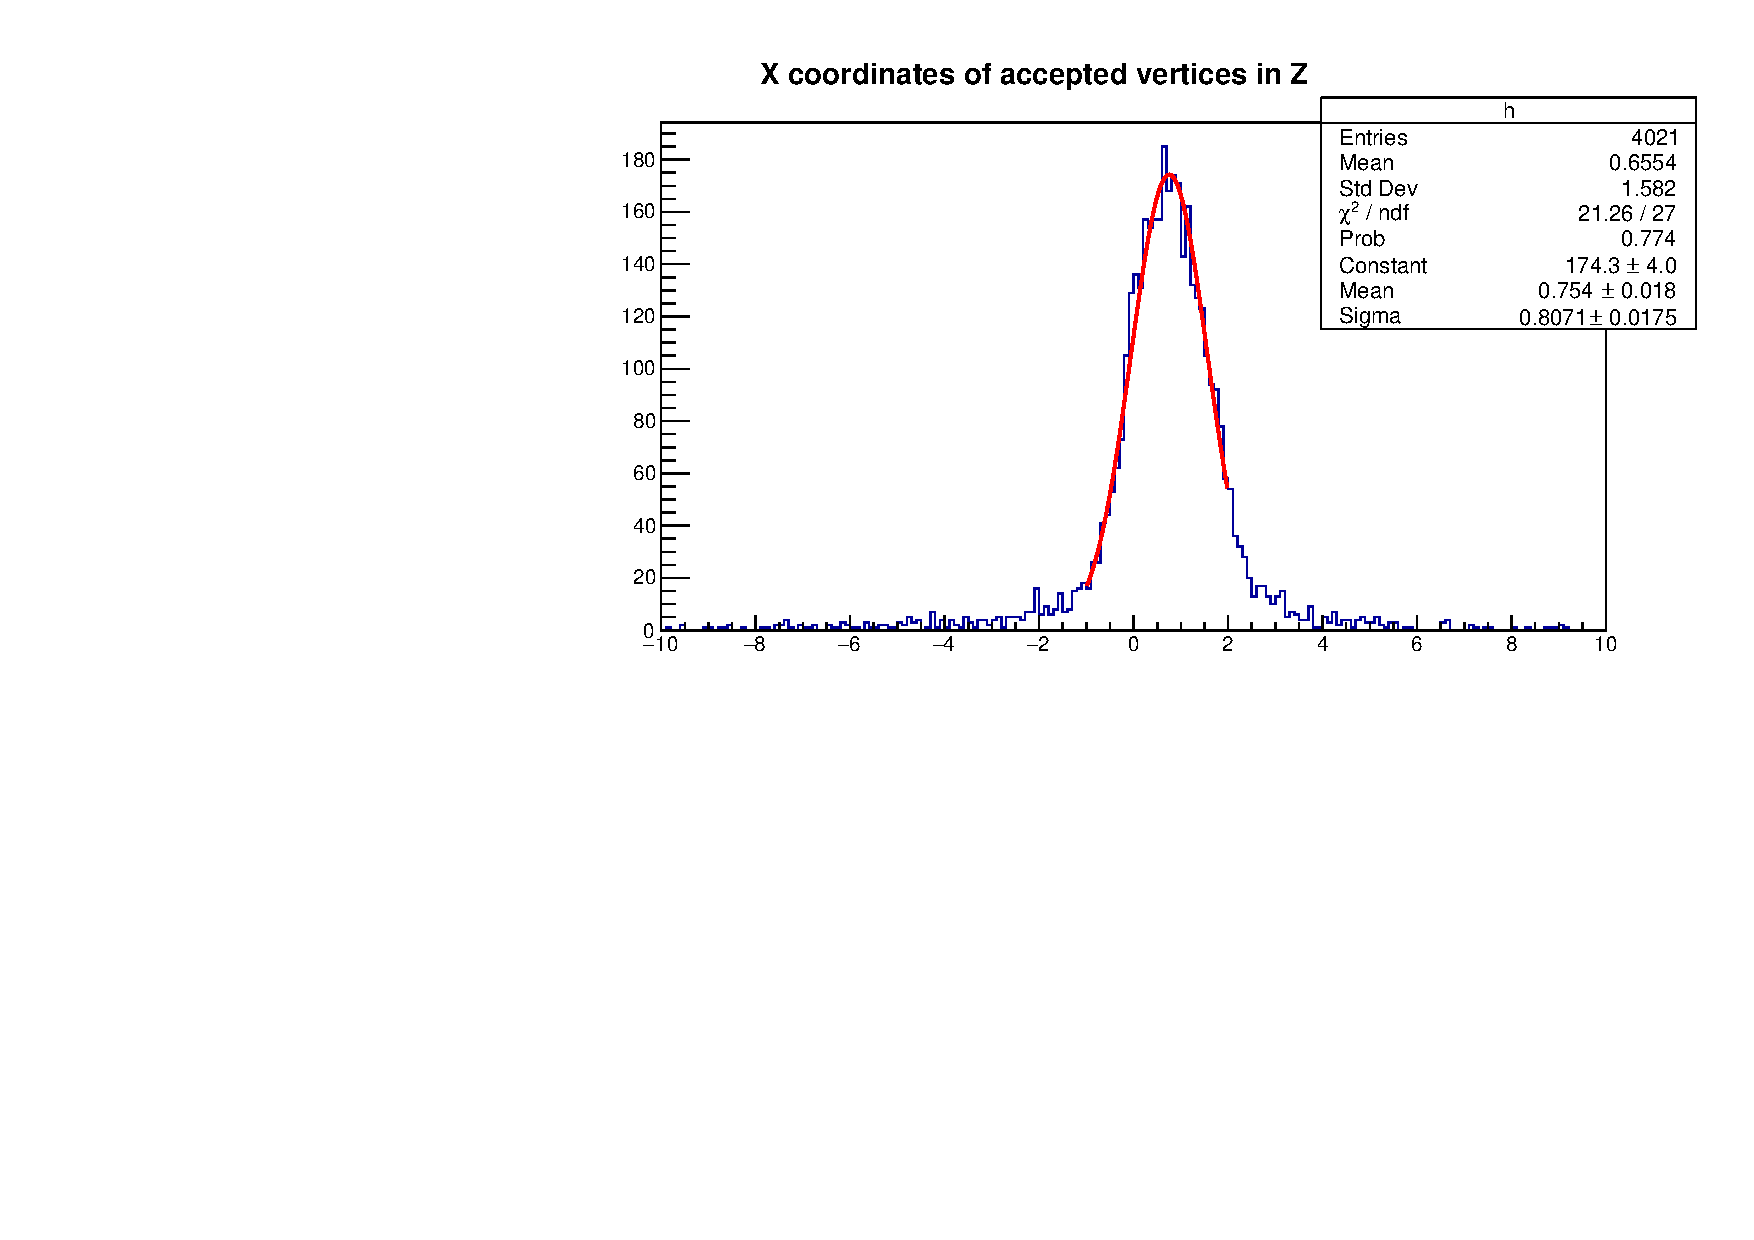
\includegraphics[width=1.\linewidth]{EmbeddingVertexX_Zcut.pdf}
            \end{figure}
             \begin{figure}[H]
              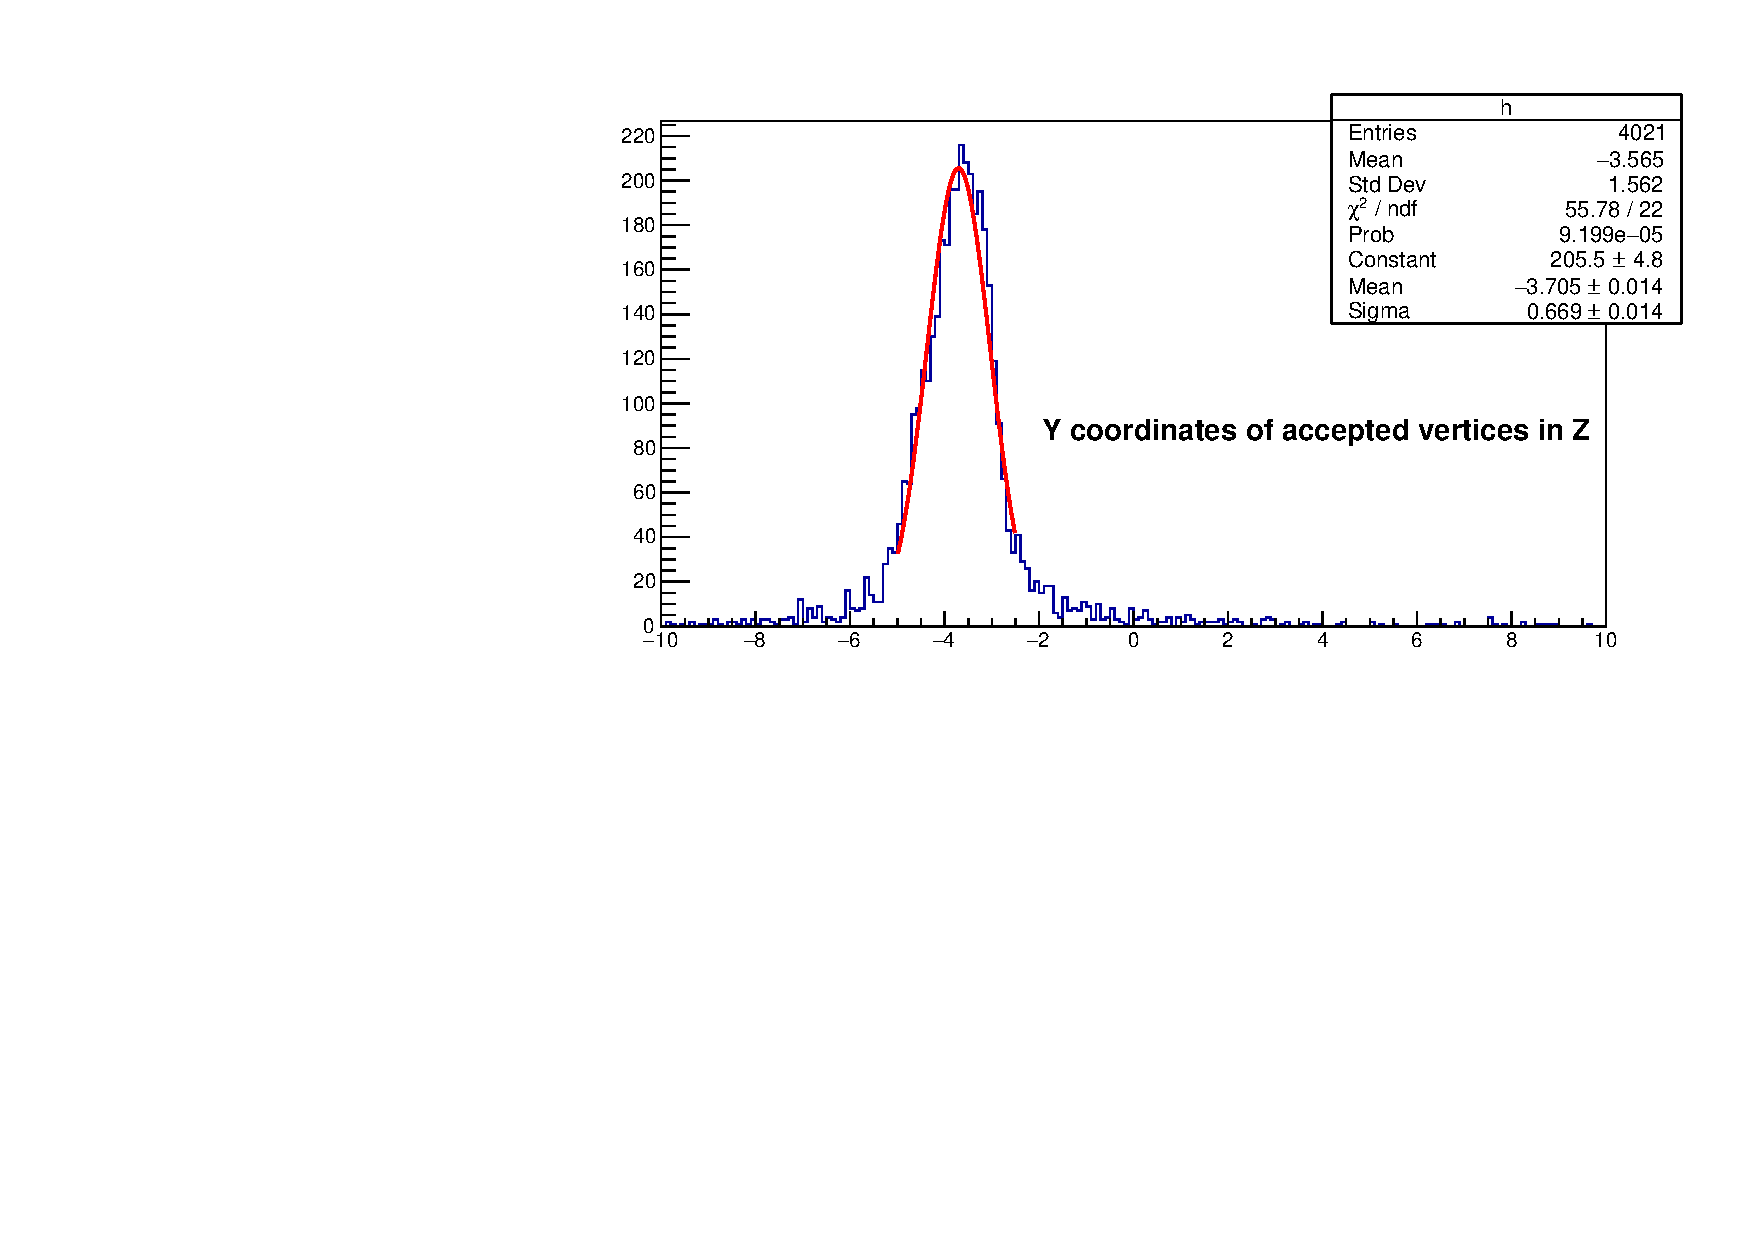
\includegraphics[width=1.\linewidth]{EmbeddingVertexY_Zcut.pdf}
            \end{figure}       
          \end{block}
        \end{columns}
      \end{frame}

      \begin{frame}
        \frametitle{\bf \centering Embedded signal for the BM@N Central Tracker}
        \begin{columns}[t]
          \column{.49\textwidth}
          \begin{figure}[H]
           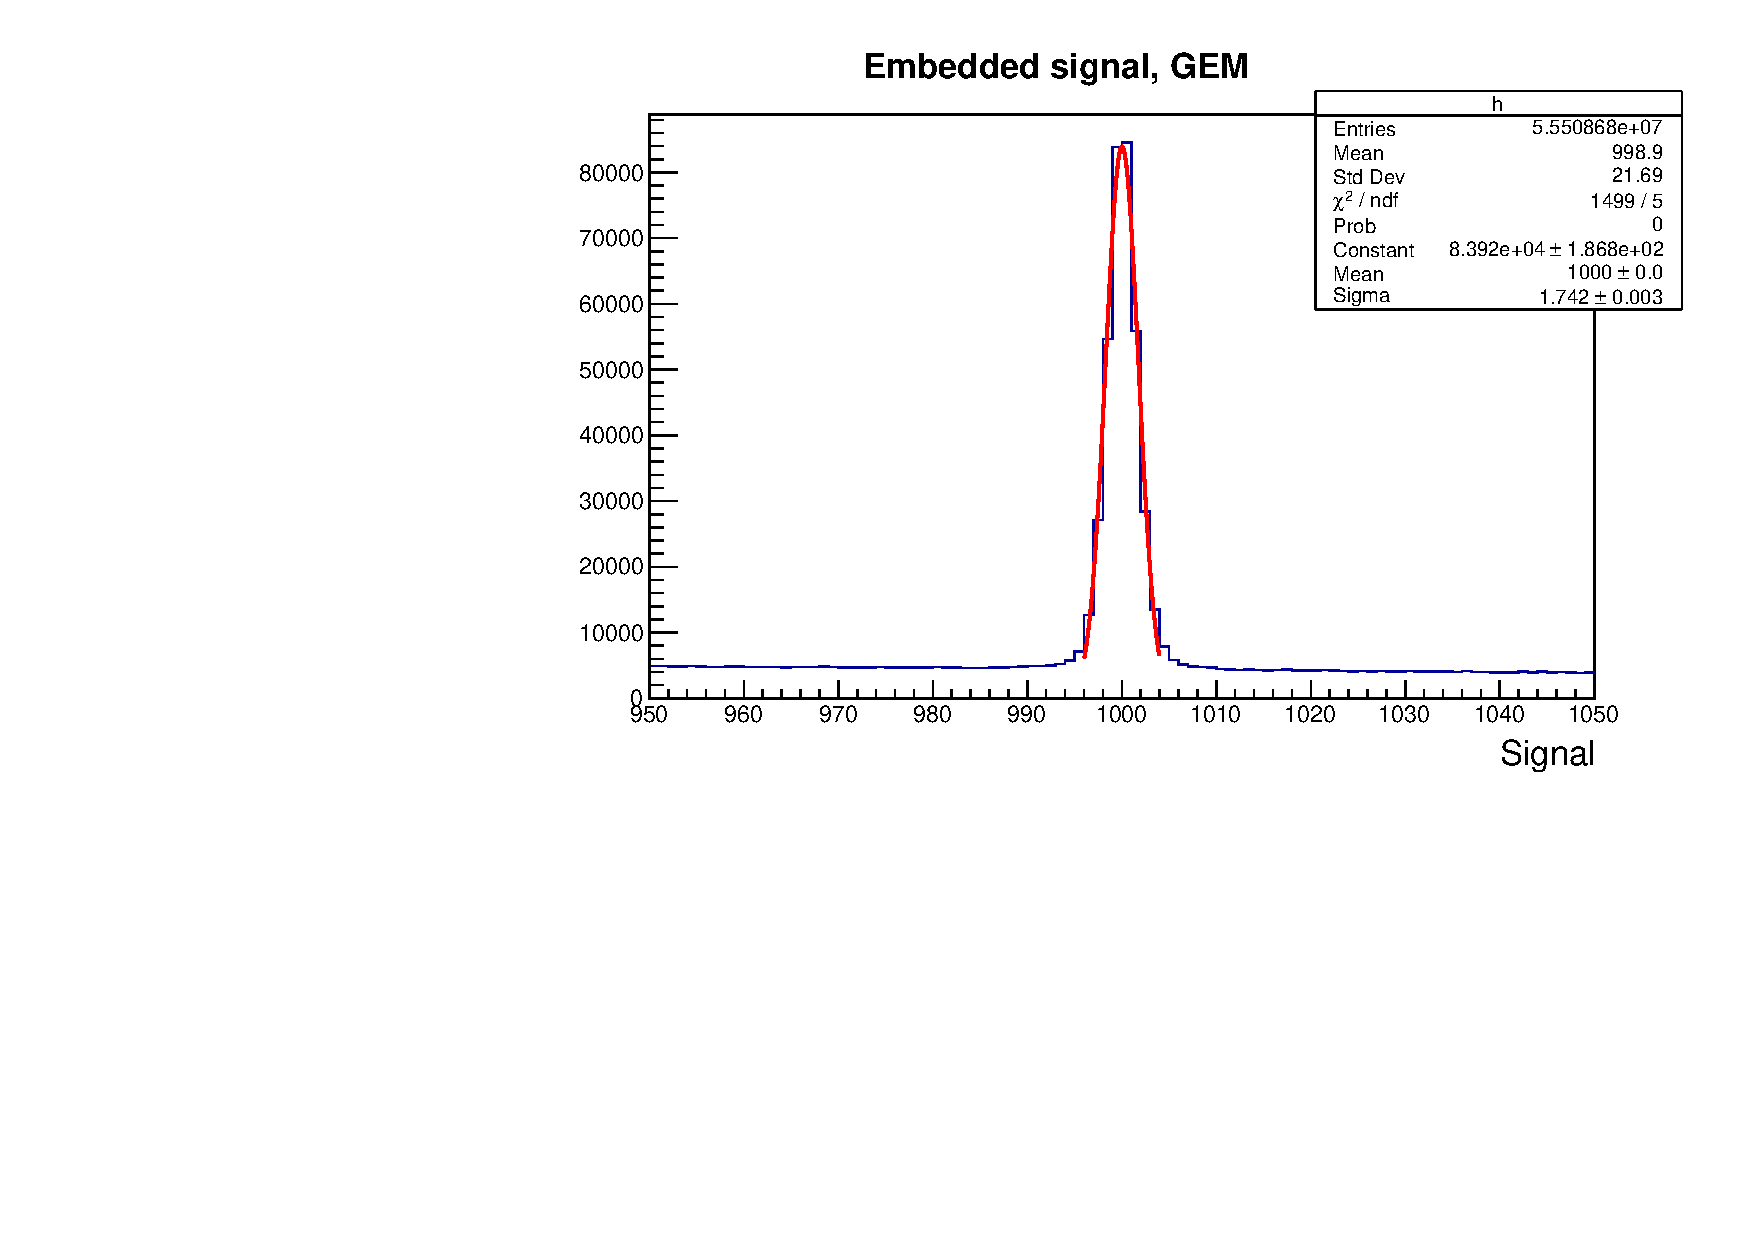
\includegraphics[width=1.\linewidth]{EmbeddedGemSignal.pdf}
          \end{figure}
          \column{.49\textwidth}
          \begin{figure}[H]
           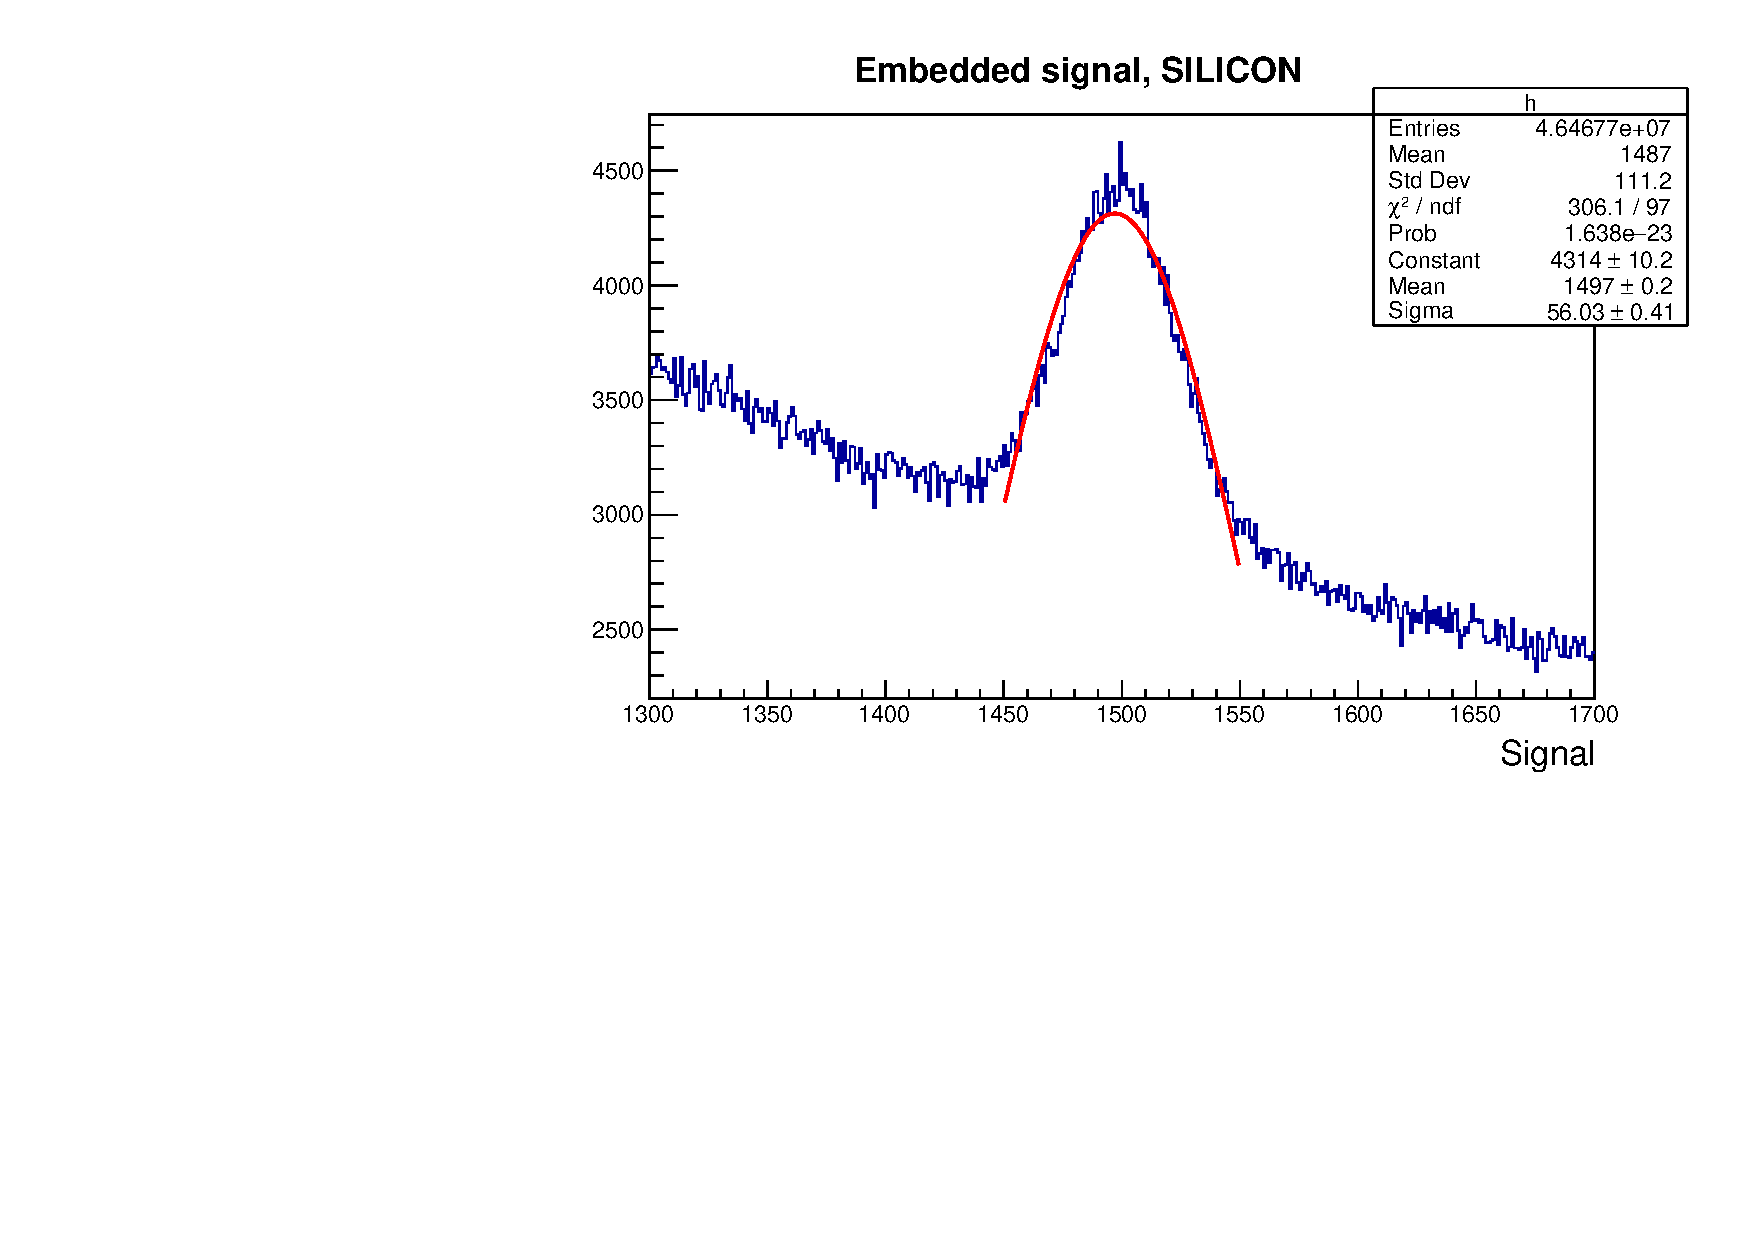
\includegraphics[width=1.\linewidth]{EmbeddedSiliconSignal.pdf}
          \end{figure}
        \end{columns}
        \begin{block}{}
          \bf
          Embedded signal for SILICON part of the tracker looks wider (if comparing with GEM) due to more significant fluctuations of
          Command Mode when decoding
        \end{block}
        
      \end{frame}
       
       \begin{frame}
         \frametitle{\bf \centering QA of the embedding procedure}
         \vskip -.83cm
         \begin{columns}[t]
           \column{.2\textwidth}
           \column{.7\textwidth}
         \begin{figure}[H]
           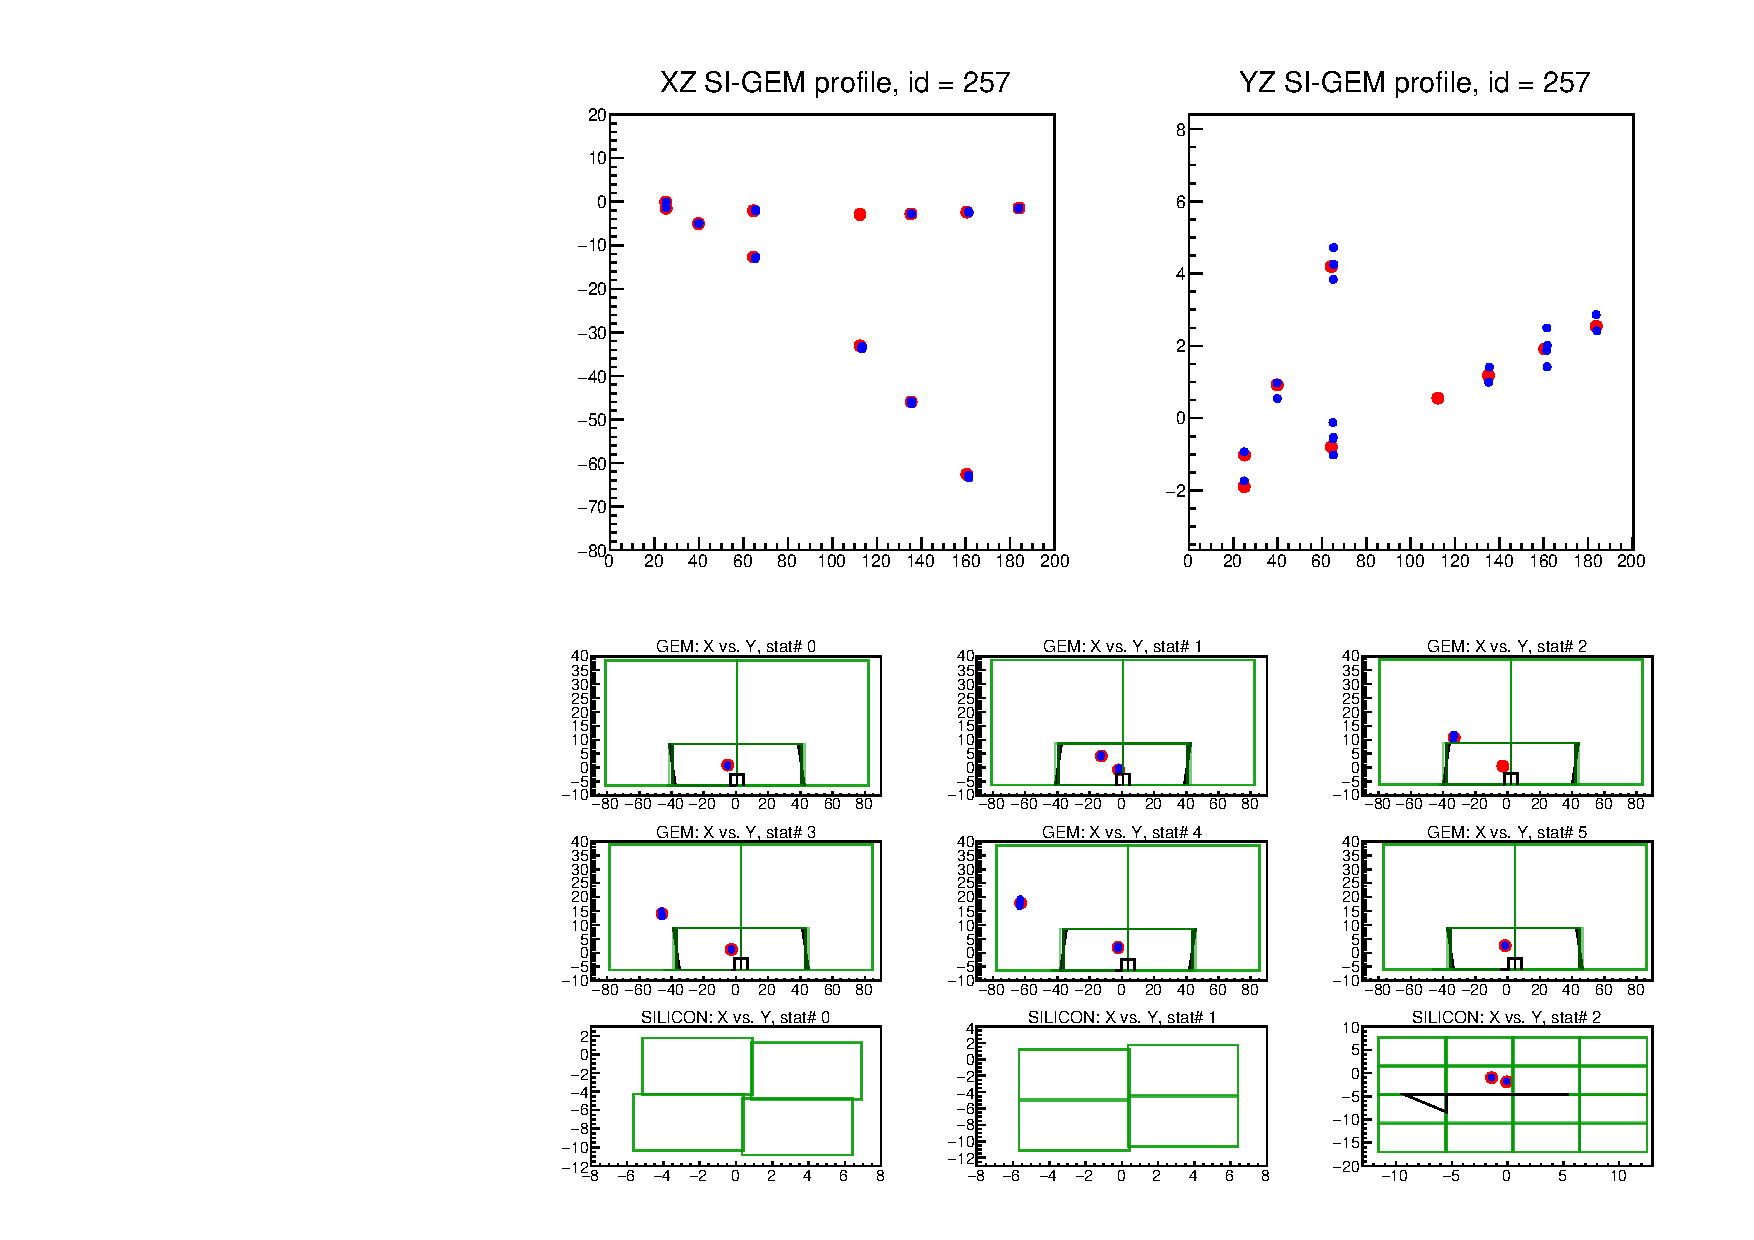
\includegraphics[width=1.\linewidth]{EmbeddingId257.pdf}
         \end{figure}
           \column{.2\textwidth}

         \end{columns}
       \end{frame}

       \begin{frame}
         \bf
         \frametitle{\bf \centering Efficiency of the embedding procedure}
         \begin{block}{}
           \begin{itemize}
           \item Calculated for different pseudorapidity ranges of $\Lambda^{0}$ to test precisely the procedure
             for different elements of the BM@N Central Tracker (stations, modules, zones)
           \item Tested different approaches to parameterizations of cluster amplitudes (signals)
             (equal amplitudes, Gaussian distribution of amplitudes)
         \end{itemize}
         \end{block}
       \end{frame}

     

         \begin{frame}
         \frametitle{\bf \centering Embedding for different $\eta$-ranges of $\Lambda^{0}$}
         \begin{columns}
           \column{.4\textwidth}
           \begin{block}{\bf \centering 1 < $\eta$ < 1.5}
             \begin{figure}[H]
             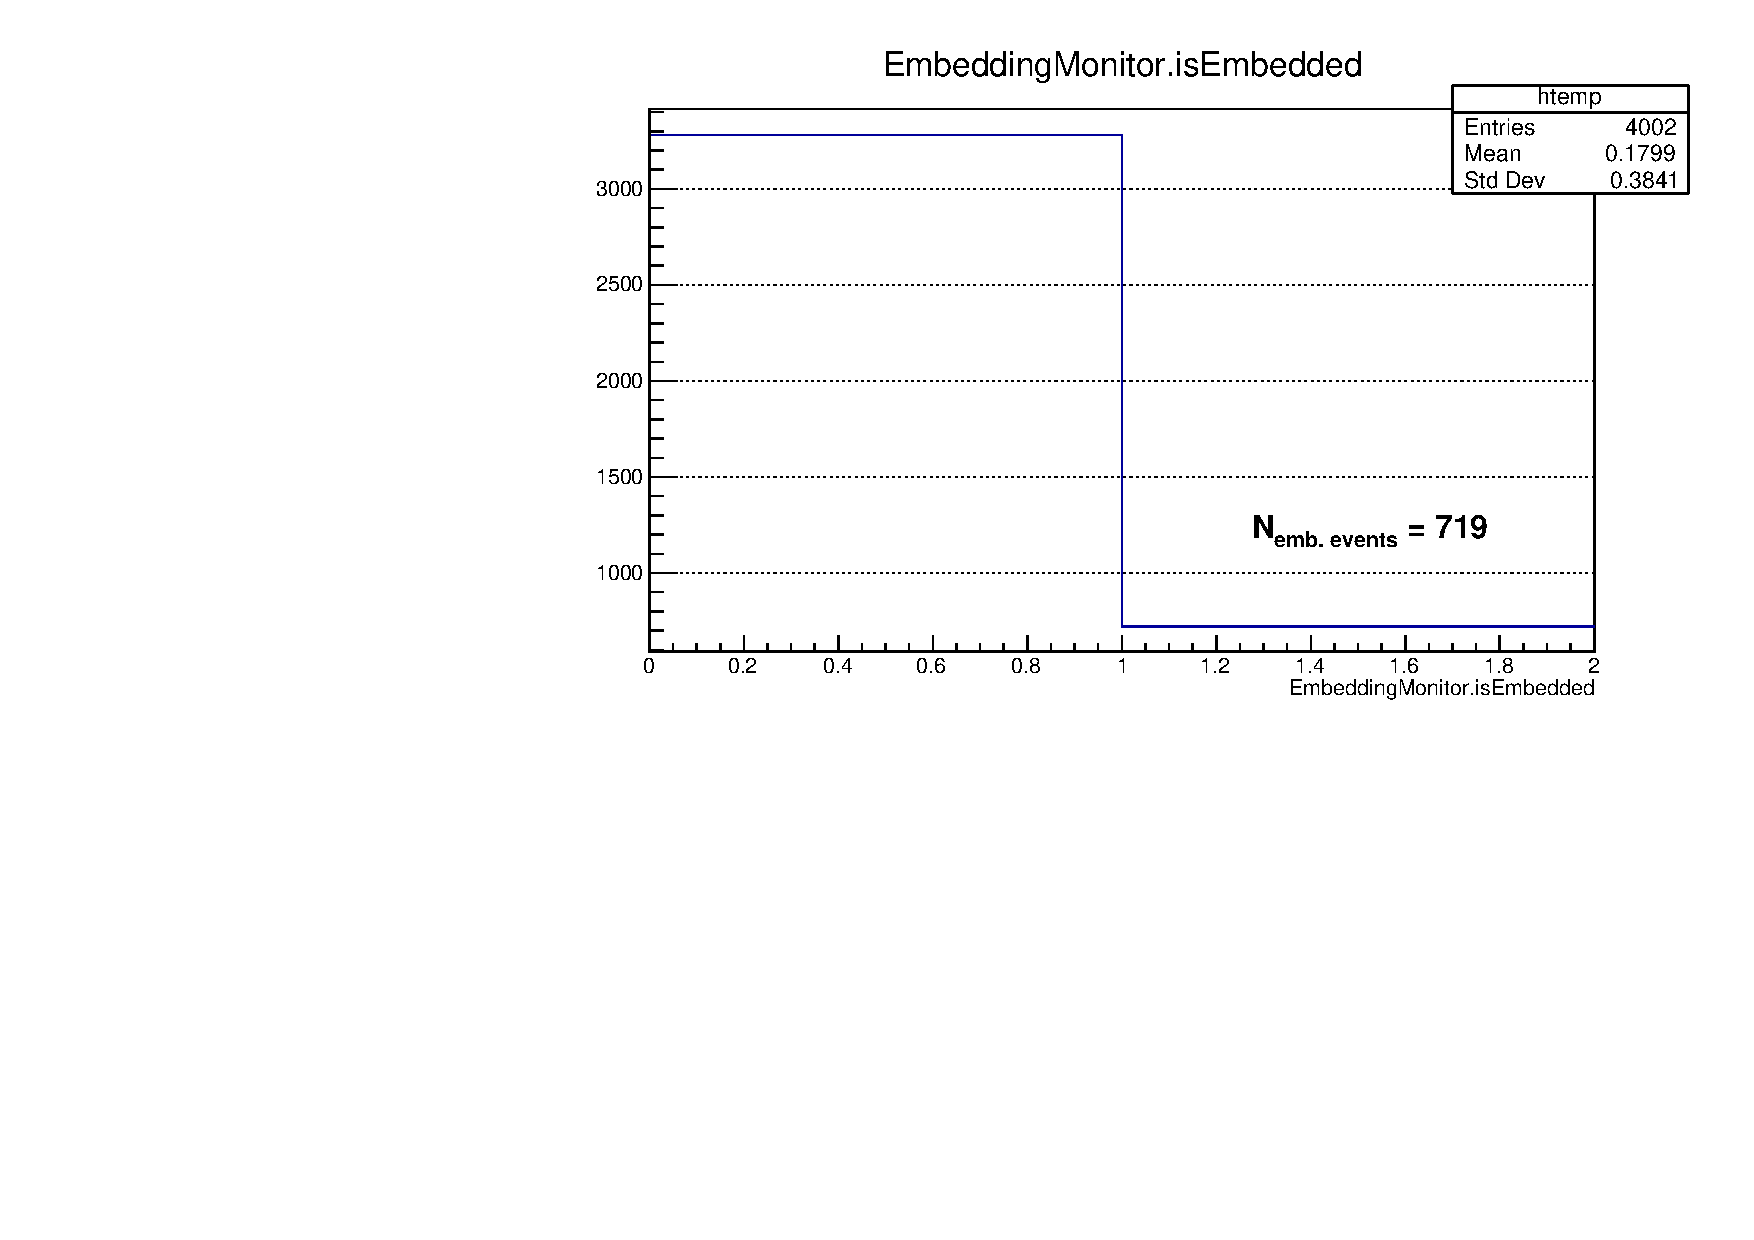
\includegraphics[width=1.\linewidth]{isEmbedded_eta_10_15.pdf}
             \end{figure}
             
           \end{block}
           \begin{block}{\bf \centering 1.5 < $\eta$ < 2}
               \begin{figure}[H]
                 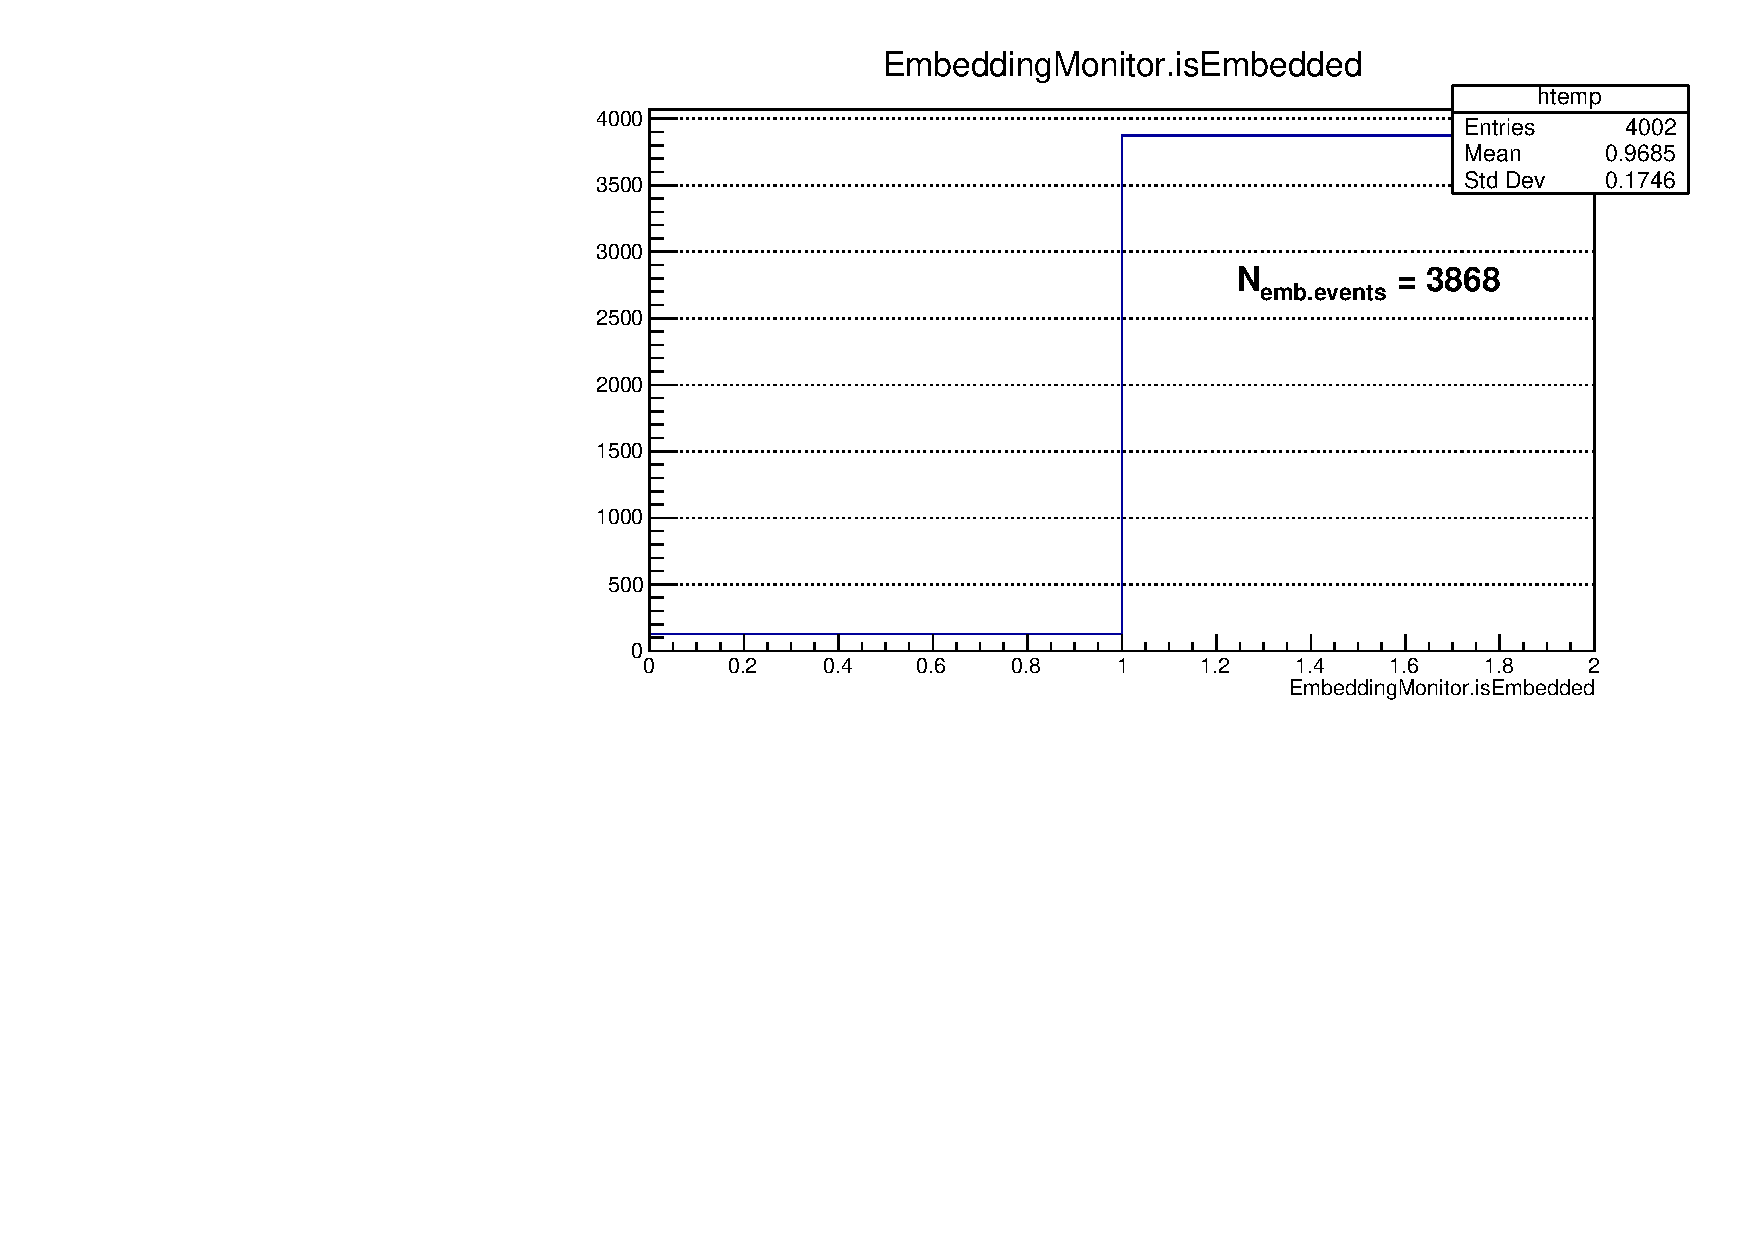
\includegraphics[width=1.\linewidth]{isEmbedded_eta_15_20.pdf}
               \end{figure}
           \end{block}

           \column{.45\textwidth}
           \begin{block}{\bf \centering 2 < $\eta$ < 3}
              \begin{figure}[H]
                 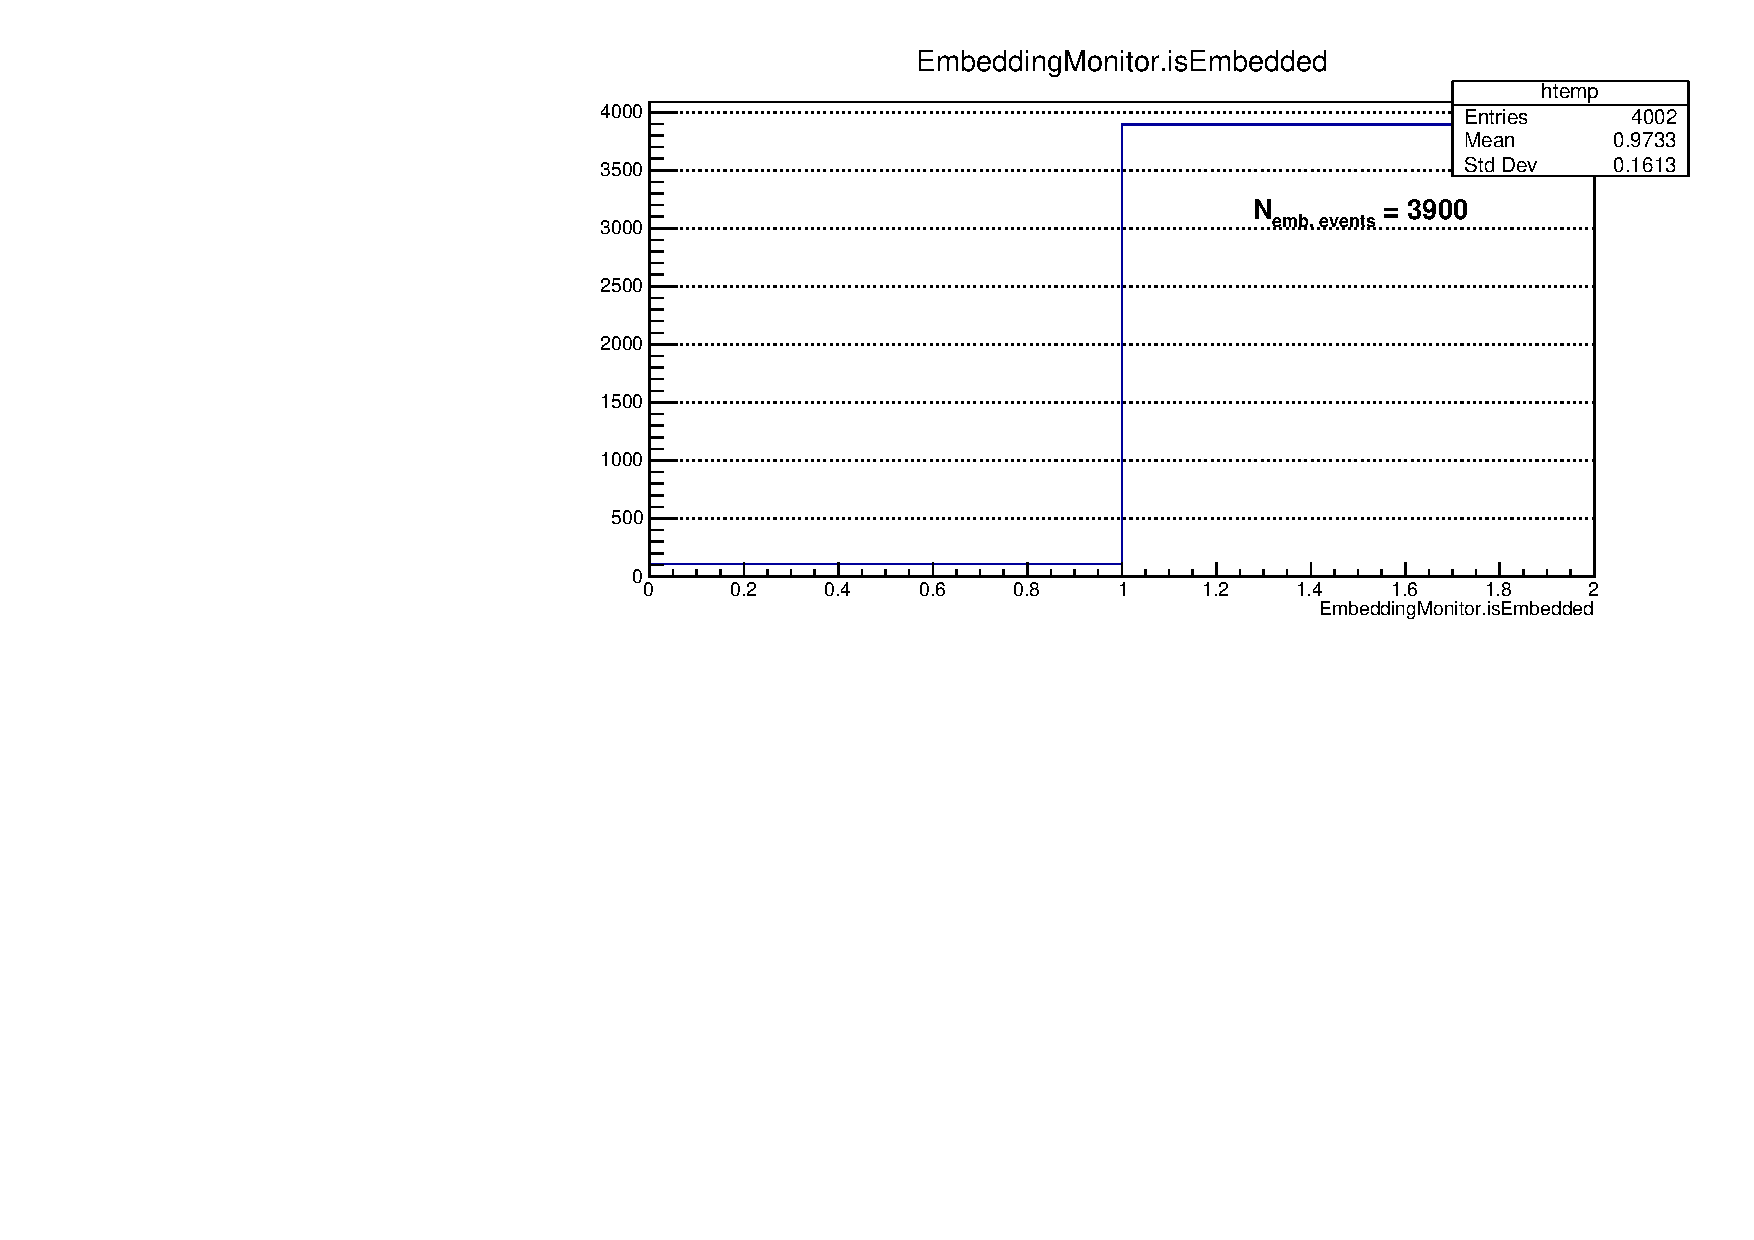
\includegraphics[width=1.\linewidth]{isEmbedded_eta_20_30.pdf}
               \end{figure}
           \end{block}
           \begin{block}{}
             \begin{itemize}
               \tiny
             \item \bf Number of events in the DST-file is {\color{red} 199000}
             \item \bf Number of events with reconstructed vertex satisfying to cuts is {\color{red} 4002}
             \item \bf Embedded particles are MC decay products (p, $\pi^{-}$) from $\Lambda^{0}$ decay
             \item \bf Each product has, at least, {\color{red} four} hits in the BM@N Central Tracker acceptance (not depending where, either GEM+SI or GEM only)
             \end{itemize}
           \end{block}         
         \end{columns}
         \end{frame}

         \begin{frame}
           \bf
           \vskip -0.25cm
           \frametitle{\bf \centering \footnotesize Efficiency of the embedding procedure integrated over all $\eta$-ranges}
           \begin{block}{\bf \centering GEM}
             \begin{figure}[H]
               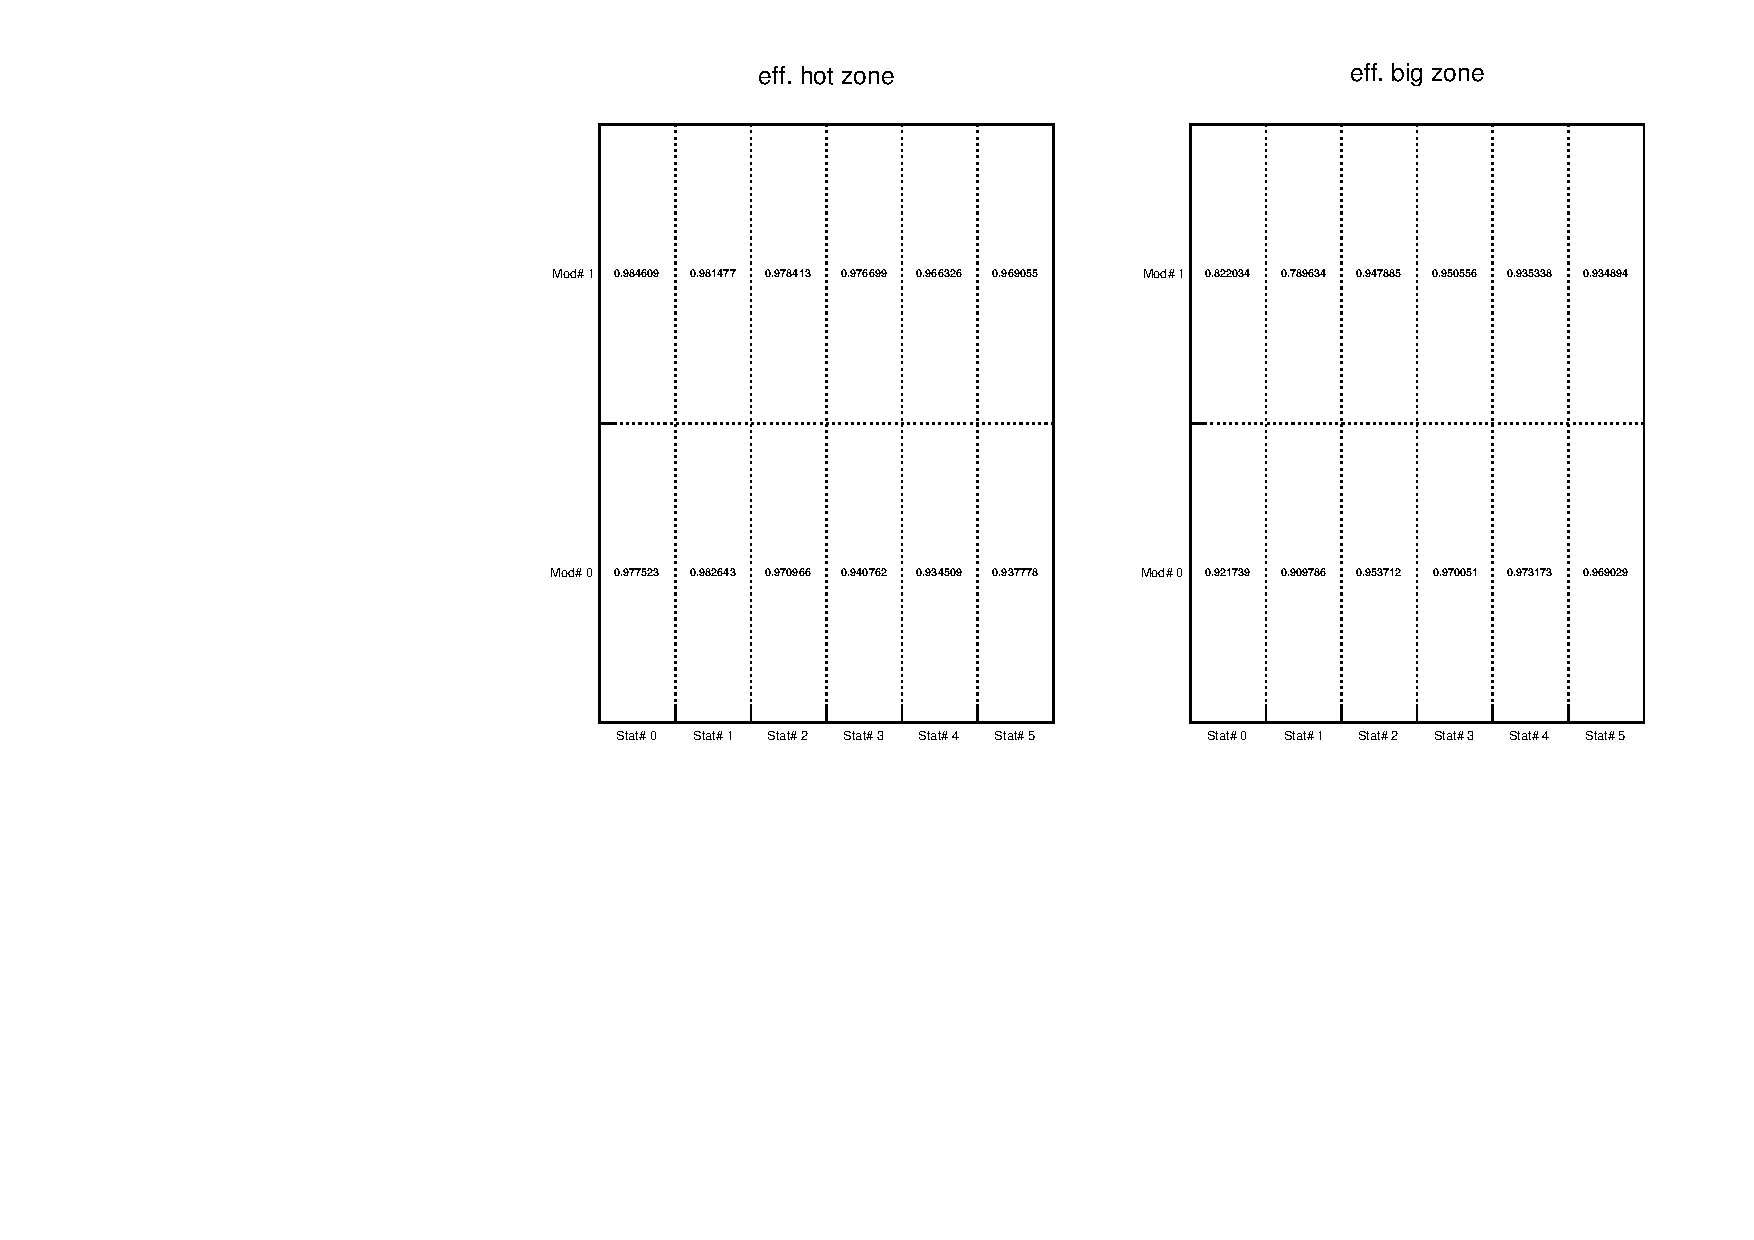
\includegraphics[width=1.\linewidth]{gemEmbHitEff_allRanges.pdf}
             \end{figure}
           \end{block}
         \end{frame}

          \begin{frame}
           \bf
           \vskip -0.25cm
           \frametitle{\bf \centering \footnotesize Efficiency of the embedding procedure integrated over all $\eta$-ranges}
           \begin{block}{\bf \centering SILICON}
             \begin{figure}[H]
               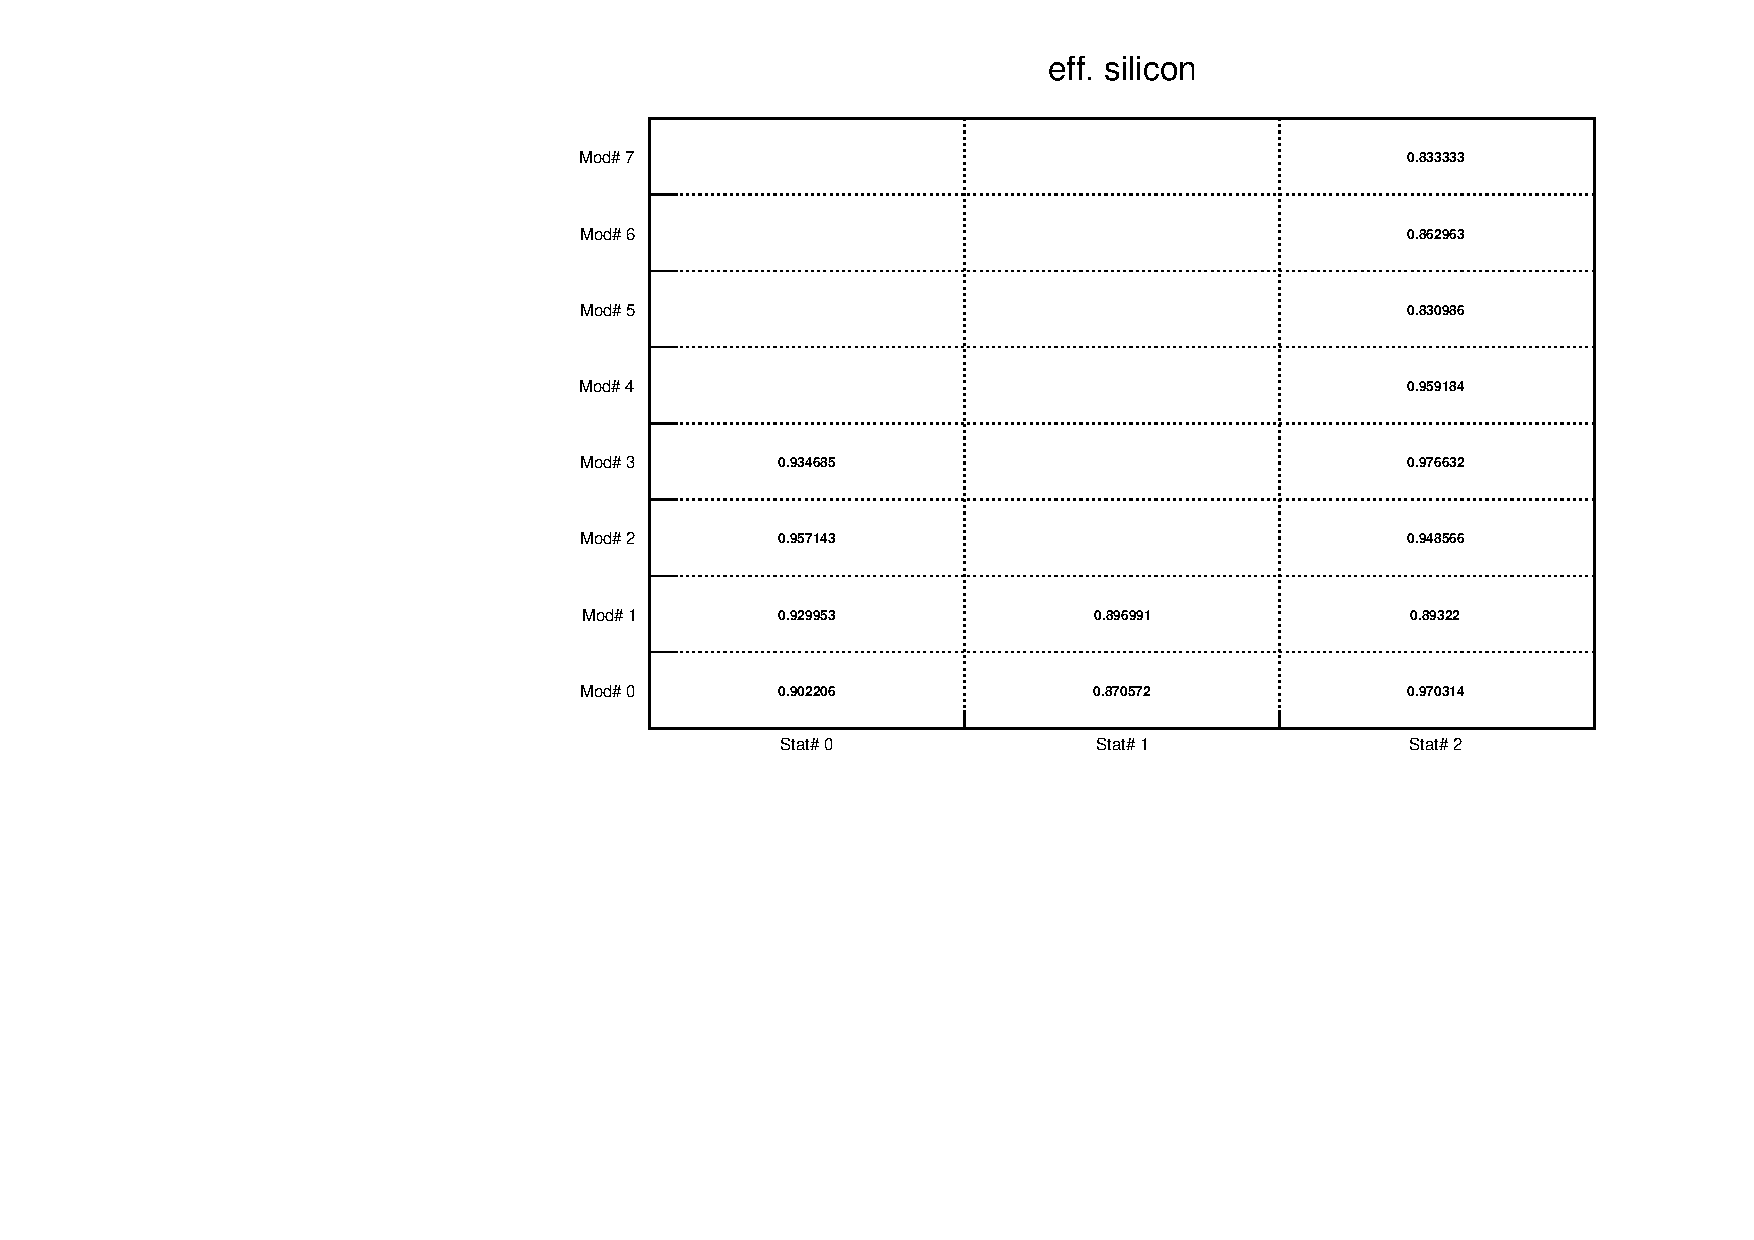
\includegraphics[width=1.\linewidth]{silEmbHitEff_allRanges.pdf}
             \end{figure}
           \end{block}
         \end{frame}

           \begin{frame}
             \frametitle{\bf \centering Parameterization of cluster amplitudes tried}          
              \begin{block}{}
                 \bf Equal amplitudes for all strips are used now by default
               \end{block}
               \begin{columns}[t]
               \column{.49\textwidth}
               \begin{block}{\bf \centering Total integral is close established value}
                 \begin{figure}[H]
                   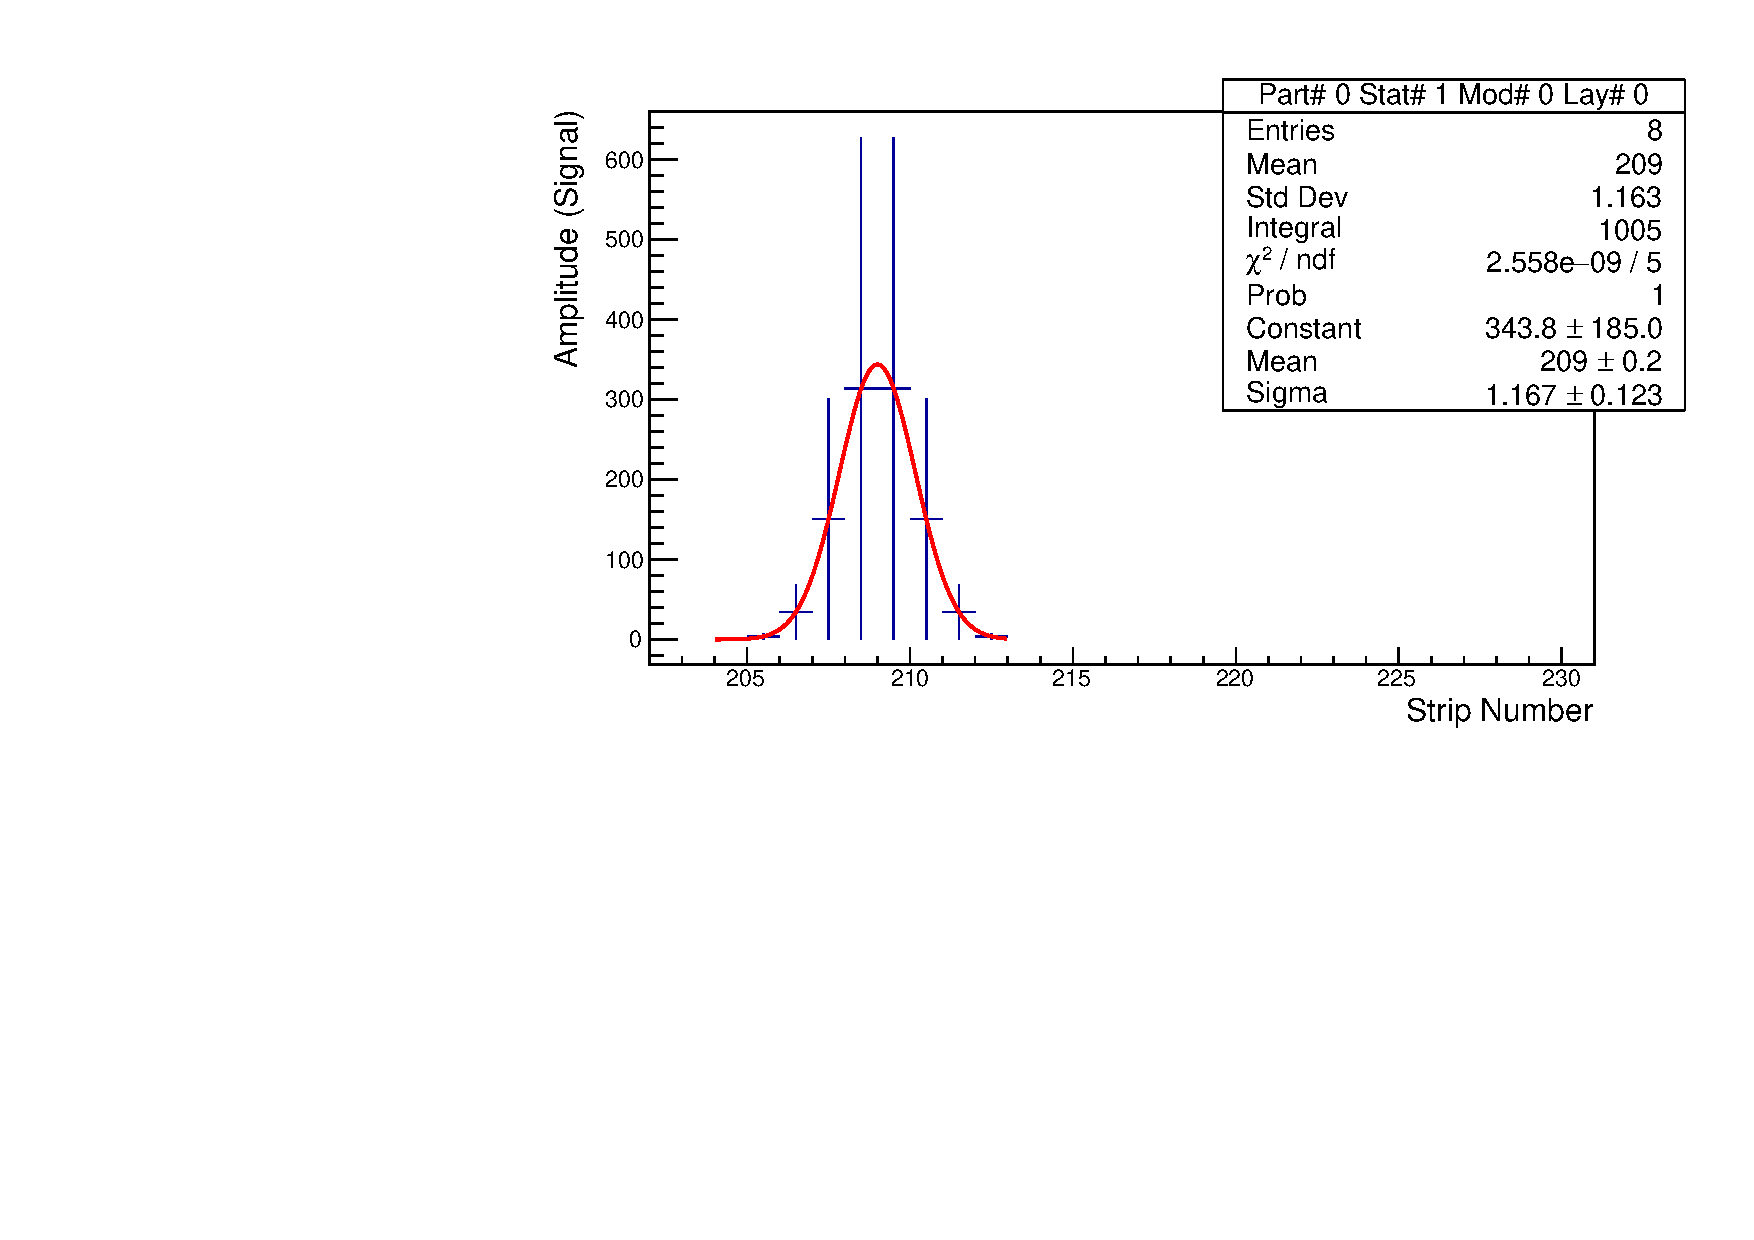
\includegraphics[width=1.\linewidth]{gausParamOverIntegral.pdf}
                 \end{figure}
               \end{block}
               \column{.49\textwidth}
               \begin{block}{\bf \centering Maximum amplitude is set to established value}
                 \begin{figure}[H]
                   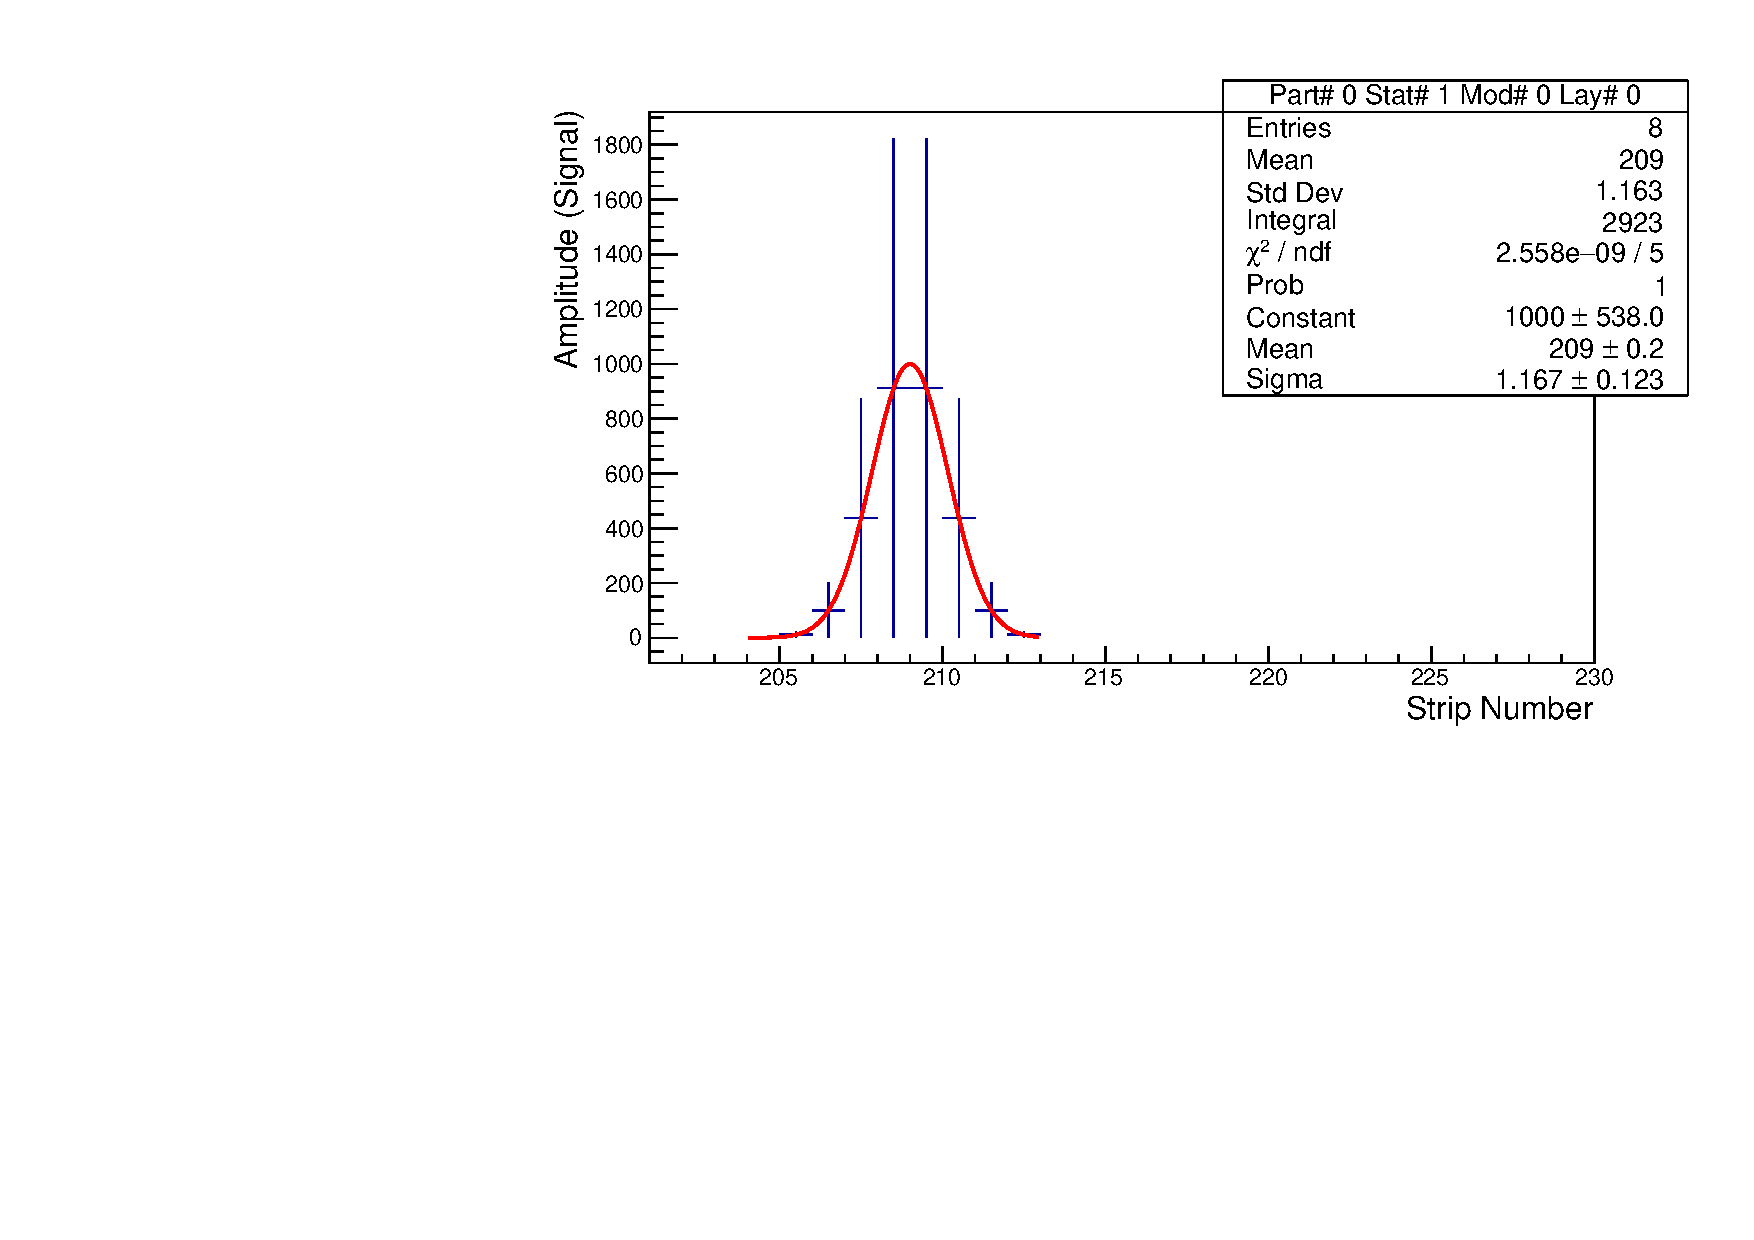
\includegraphics[width=1.\linewidth]{gausParamOverMaxValue.pdf}
                 \end{figure}
               \end{block}
               \end{columns}
               \begin{block}{}
                 \bf \color{blue} At the moment, no one additional parameterization used did not increase efficiency in case of wide clusters :(
               \end{block}
           \end{frame}

           \begin{frame}
             \frametitle{\bf \centering Efficiency of the procedure}
             \begin{block}{\bf \centering }
               \begin{figure}[H]
                 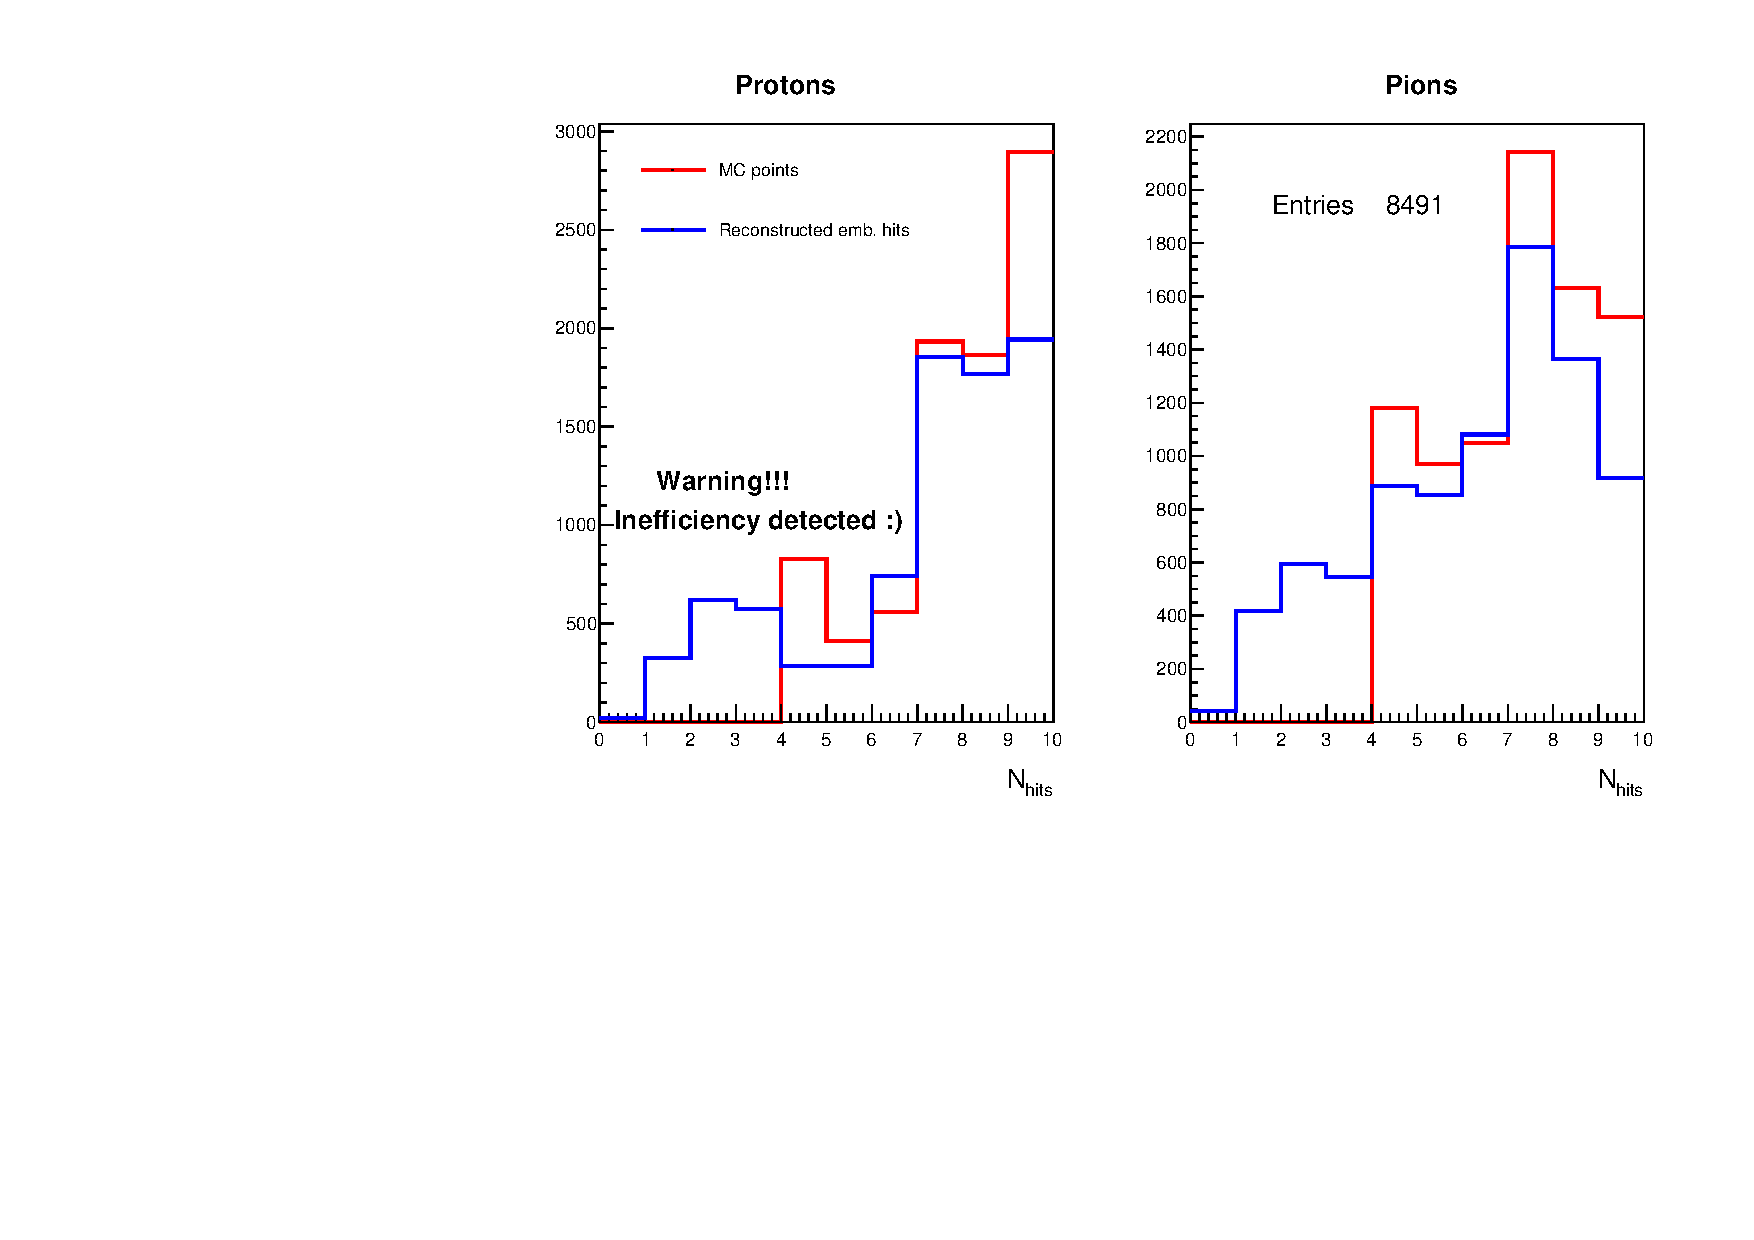
\includegraphics[width=1.\linewidth]{EmbeddingHitRecoEff.pdf}
               \end{figure}
             \end{block}
           \end{frame}

           \begin{frame}
             \frametitle{\bf \centering TODO list:}
             \bf
             \begin{itemize}
             \item {\color{red} To find out why we have a visible inefficiency in big zones, especially, for first two GEM stations of the BM@N Central Tracker}
             \item When being done, try to do a preliminary set of tracking to reconstruct $\Lambda^{0}$ decay products with a high efficiency
             \item After that, try to perform a correct scaling of embedded signals (from digitizer) to those ones got from experimental data
             \item Finally, measure efficiency for both procedures, embedding and tracking
             \item Further tests aiming at $\Lambda^{0}$ reconstruction with improved tracking using existing code \\
               {(\scriptsize \$VMCWORKDIR/physics/particles/BmnTwoParticleDecay.h})
             \item More unknown as yet tests to be done :)
               
               
             \end{itemize}
           \end{frame}
         
      
      
      \end{document}
      
